%2multibyte Version: 5.50.0.2960 CodePage: 65001
% !TeX root = ./Slides_Lez_12_Dualita_ALM_Deterministico.tex
% ------------------------------------------------------------
% Slides Lezione 12 - Dualit\`{a} e ALM deterministico
% Progetto MQF - Metodi Quantitativi per la Finanza
% Macro matematiche ufficiali del progetto MQF
% Coerenti con MQF_Notazione.tex
% ------------------------------------------------------------
% Fallback utile per compilazione esterna se qualche titolo resta scritto come \QTR.
% Scientific WorkPlace usa \QTR internamente; in Beamer \QTR{frametitle}{Titolo}
% deve espandersi in \frametitle{Titolo}.

\documentclass[handout]{beamer}%
\usepackage{mathpazo}
%\usepackage{hyperref}
\usepackage{multimedia}
\usepackage{amsmath}
\usepackage{amsfonts}
\usepackage{amssymb}
\usepackage{graphicx}%
\setcounter{MaxMatrixCols}{30}
%TCIDATA{OutputFilter=latex2.dll}
%TCIDATA{Version=5.50.0.2960}
%TCIDATA{Codepage=65001}
%TCIDATA{CSTFile=beamer.cst}
%TCIDATA{<META NAME="GraphicsSave" CONTENT="32">}
%TCIDATA{<META NAME="SaveForMode" CONTENT="2">}
%TCIDATA{BibliographyScheme=Manual}
%TCIDATA{<META NAME="DocumentShell" CONTENT="Other Documents\SW\Slides - Beamer">}
%BeginMSIPreambleData
\providecommand{\U}[1]{\protect\rule{.1in}{.1in}}
%EndMSIPreambleData
\newenvironment{stepenumerate}{\begin{enumerate}[<+->]}{\end{enumerate}}
\newenvironment{stepitemize}{\begin{itemize}[<+->]}{\end{itemize} }
\newenvironment{stepenumeratewithalert}{\begin{enumerate}[<+-| alert@+>]}{\end{enumerate}}
\newenvironment{stepitemizewithalert}{\begin{itemize}[<+-| alert@+>]}{\end{itemize} }
\usetheme{Madrid}
\providecommand{\R}{\mathbb{R}}
\providecommand{\N}{\mathbb{N}}
\providecommand{\E}{\mathbb{E}}
\providecommand{\Prob}{\mathbb{P}}
\providecommand{\Q}{\mathbb{Q}}
\providecommand{\F}{\mathcal{F}}
\providecommand{\B}{\mathcal{B}}
\providecommand{\G}{\mathcal{G}}
\providecommand{\Var}{\operatorname{Var}}
\providecommand{\Cov}{\operatorname{Cov}}
\providecommand{\VaR}{\operatorname{VaR}}
\providecommand{\CVaR}{\operatorname{CVaR}}
\providecommand{\argmin}{\operatorname*{arg\,min}}
\providecommand{\argmax}{\operatorname*{arg\,max}}
\providecommand{\EVPI}{\operatorname{EVPI}}
\providecommand{\VSS}{\operatorname{VSS}}
\providecommand{\QTR}[2]{\csname #1\endcsname{#2}}
%BeginMSIPreambleData
\ifx\pdfoutput\relax\let\pdfoutput=\undefined\fi
\newcount\msipdfoutput
\ifx\pdfoutput\undefined\else
\ifcase\pdfoutput\else
\msipdfoutput=1
\ifx\paperwidth\undefined\else
\ifdim\paperheight=0pt\relax\else\pdfpageheight\paperheight\fi
\ifdim\paperwidth=0pt\relax\else\pdfpagewidth\paperwidth\fi
\fi\fi\fi
%EndMSIPreambleData


\title[Dualit\`{a} e ALM]{Lezione 12 -- Dualit\`{a} e Asset--Liability
Management deterministico}
\subtitle{Metodi Quantitativi per la Finanza}
\author[P. Falbo, C. Pelizzari]{{\LARGE Paolo Falbo, Cristian Pelizzari}}
\institute[]{{\large Dipartimento di Economia e Management}}
\date[]{}
\titlegraphic{

\includegraphics[width=3.3cm]{../graphics/logo-Unibs-esteso.png}
}

\begin{document}
\maketitle

%****************************************

\section{Apertura}

\subsection{Il modello SVB in una pagina}%

%TCIMACRO{\TeXButton{BeginFrame}{\begin{frame}}}%
%BeginExpansion
\begin{frame}%
%EndExpansion

\QTR{frametitle}{Richiamo: il modello SVB stilizzato}

%TCIMACRO{\TeXButton{Transparency}{\setbeamercovered{transparent=20}}}%
%BeginExpansion
\setbeamercovered{transparent=20}%
%EndExpansion

Quattro variabili decisionali: quanto destinare a ciascuna classe di attivo,
a partire da risorse iniziali $A_0=100$.

\medskip

{\small
\[
\begin{array}{c|l|c|c|c}
\hline
 & \mbox{classe di attivo} & c_j & \ell_j & q_j\\
\hline
x_1 & \mbox{cassa e riserve}          & 0.010 & 0    & 1.00\\
x_2 & \mbox{titoli a breve scadenza}  & 0.025 & 0.02 & 0.90\\
x_3 & \mbox{titoli a lunga scadenza}  & 0.040 & 0.15 & 0.50\\
x_4 & \mbox{prestiti e impieghi}      & 0.050 & 0.08 & 0.20\\
\hline
\end{array}
\]
}

\medskip

{\small
\[
\begin{array}{ll}
\max & c'x\\[4pt]
\mbox{s.a}
& x_1+x_2+x_3+x_4=100
\qquad\mbox{(bilancio)}\\[2pt]
& q'x\geq55
\qquad\qquad\qquad\quad\;\;\mbox{(liquidit\`{a})}\\[2pt]
& \ell'x\leq7
\qquad\qquad\qquad\quad\;\;\;\mbox{(perdita sotto stress)}\\[2pt]
& x_3\leq30
\qquad\qquad\qquad\quad\;\;\;\mbox{(concentrazione)}\\[2pt]
& x\geq0
\end{array}
\]
}

\medskip

{\footnotesize Redditivit\`{a} e liquidit\`{a} vanno in direzioni opposte: la
cassa \`{e} perfettamente liquida ma rende $0.010$, i prestiti rendono
$0.050$ ma liberano solo $0.20$ per unit\`{a}.}

%TCIMACRO{\TeXButton{Transition: Box Out}{\transboxout}}%
%BeginExpansion
\transboxout%
%EndExpansion
%TCIMACRO{\TeXButton{EndFrame}{\end{frame}}}%
%BeginExpansion
\end{frame}%
%EndExpansion

%****************************************

\subsection{Il vincolo ha un prezzo}%

%TCIMACRO{\TeXButton{BeginFrame}{\begin{frame}}}%
%BeginExpansion
\begin{frame}%
%EndExpansion

\QTR{frametitle}{Dove eravamo: il vincolo ha un prezzo}

%TCIMACRO{\TeXButton{Transparency}{\setbeamercovered{transparent=20}}}%
%BeginExpansion
\setbeamercovered{transparent=20}%
%EndExpansion

Nel Capitolo~11 la banca sceglie la composizione dell'attivo che massimizza
il risultato economico, rispettando bilancio, liquidit\`{a}, perdita sotto
stress e concentrazione.

\medskip

{\small
\[
x^{*}
\approx
\left(
0,\;41.045,\;20.896,\;38.060
\right)',
\qquad
z^{*}
\approx
3.765.
\]
}

\medskip

\begin{stepitemize}
\item Due vincoli risultano \textbf{attivi}: il requisito di liquidit\`{a} e
il limite alla perdita sotto stress. Il limite di concentrazione conserva
invece un margine.

\item Irrigidendo di poco il requisito e \emph{risolvendo di nuovo} il
modello, abbiamo misurato di quanto peggiora il risultato:

{\small
\[
\Delta z^{*}
\approx
-\lambda_{Q}^{*}\,\Delta Q_{\min},
\qquad
\lambda_{Q}^{*}
\approx
0.03507.
\]
}

\item Quel numero non era nella formulazione del problema: \`{e} emerso da un
calcolo ripetuto.
\end{stepitemize}

%TCIMACRO{\TeXButton{Transition: Box Out}{\transboxout}}%
%BeginExpansion
\transboxout%
%EndExpansion
%TCIMACRO{\TeXButton{EndFrame}{\end{frame}}}%
%BeginExpansion
\end{frame}%
%EndExpansion

%****************************************

\subsection{Le due domande della lezione}%

%TCIMACRO{\TeXButton{BeginFrame}{\begin{frame}}}%
%BeginExpansion
\begin{frame}%
%EndExpansion

\QTR{frametitle}{Le due domande della lezione}

%TCIMACRO{\TeXButton{Transparency}{\setbeamercovered{transparent=20}}}%
%BeginExpansion
\setbeamercovered{transparent=20}%
%EndExpansion

\begin{stepenumerate}
\item [1.] \textbf{Da dove viene quel prezzo?}

Esiste un secondo problema lineare che produce \emph{tutti} i prezzi in una
sola soluzione, senza ricalcolare l'ottimo un requisito alla volta: il
\textbf{problema duale}.

\item [2.] \textbf{\`{E} davvero un solo prezzo?}

Nel modello statico la liquidit\`{a} \`{e} misurata da un unico requisito
aggregato,

{\small
\[
\sum_{j=1}^{4}q_jx_j\geq Q_{\min}.
\]
}

Il coefficiente $q_j$ dice \emph{quanta} liquidit\`{a} produce l'attivit\`{a}
$j$, ma non dice \emph{quando} quella liquidit\`{a} diventa disponibile.
\end{stepenumerate}

\medskip

{\small
\[
\boxed{
\mbox{quanto}
\qquad\longrightarrow\qquad
\mbox{quanto e quando}
}
\]
}

%TCIMACRO{\TeXButton{Transition: Box Out}{\transboxout}}%
%BeginExpansion
\transboxout%
%EndExpansion
%TCIMACRO{\TeXButton{EndFrame}{\end{frame}}}%
%BeginExpansion
\end{frame}%
%EndExpansion

%****************************************

\subsection{Percorso della lezione}%

%TCIMACRO{\TeXButton{BeginFrame}{\begin{frame}}}%
%BeginExpansion
\begin{frame}%
%EndExpansion

\QTR{frametitle}{Percorso della lezione}

%TCIMACRO{\TeXButton{Transparency}{\setbeamercovered{transparent=20}}}%
%BeginExpansion
\setbeamercovered{transparent=20}%
%EndExpansion

\begin{stepenumerate}
\item [1.] \textbf{Costruire il duale}: da dove nascono i prezzi impliciti dei
vincoli, e perch\'{e} il valore del duale coincide con quello del primale.

\item [2.] \textbf{Distribuire nel tempo}: i cash flow prodotti dall'attivo e
i fabbisogni collocati alle diverse date.

\item [3.] \textbf{Collegare le date}: la liquidit\`{a} che si trasferisce al
periodo successivo e il funding che anticipa risorse dal futuro.

\item [4.] \textbf{Risolvere}: il caso SVB multiperiodale, e che cosa accade
alla composizione ottima del Capitolo~11.

\item [5.] \textbf{Leggere i prezzi per scadenza}: un valore marginale della
liquidit\`{a} per ciascuna data.
\end{stepenumerate}

\medskip

\begin{center}
{\small \emph{Chiave di lettura: la liquidit\`{a} non ha un prezzo, ne ha uno
per ogni data.}}
\end{center}

%TCIMACRO{\TeXButton{Transition: Box Out}{\transboxout}}%
%BeginExpansion
\transboxout%
%EndExpansion
%TCIMACRO{\TeXButton{EndFrame}{\end{frame}}}%
%BeginExpansion
\end{frame}%
%EndExpansion

%****************************************
\section{Dualit\`{a} e prezzi impliciti}

\subsection{Un problema di valutazione}%
 
%TCIMACRO{\TeXButton{BeginFrame}{\begin{frame}}}%
%BeginExpansion
\begin{frame}%
%EndExpansion
 
\QTR{frametitle}{Un secondo problema: valutare le risorse}
 
%TCIMACRO{\TeXButton{Transparency}{\setbeamercovered{transparent=20}}}%
%BeginExpansion
\setbeamercovered{transparent=20}%
%EndExpansion
 
Accanto alla domanda \emph{quale composizione scegliere}, poniamone una
diversa: \textbf{quanto vale, per la banca, ciascuna risorsa e ciascun
requisito?}
 
\medskip
 
\begin{stepitemize}
\item Attribuiamo un prezzo implicito $\lambda_i$ a ogni vincolo.
 
\item I prezzi devono essere \textbf{coerenti}: per nessuna classe di attivo
il valore delle risorse impiegate pu\`{o} risultare inferiore al contributo
economico che essa produce.
 
\item Fra tutti i sistemi di prezzi coerenti, scegliamo quello che attribuisce
alle risorse il \textbf{valore complessivo minimo}.
\end{stepitemize}
 
\medskip
 
{\small
\[
\begin{array}{lll}
\mbox{primale} & \displaystyle\max_x c'x &
\mbox{soggetto a }Ax\leq b,\quad x\geq0
\\[8pt]
\mbox{duale} & \displaystyle\min_{\lambda} b'\lambda &
\mbox{soggetto a }A'\lambda\geq c,\quad \lambda\geq0
\end{array}
\]
}
 
%TCIMACRO{\TeXButton{Transition: Box Out}{\transboxout}}%
%BeginExpansion
\transboxout%
%EndExpansion
%TCIMACRO{\TeXButton{EndFrame}{\end{frame}}}%
%BeginExpansion
\end{frame}%
%EndExpansion
 
%****************************************
 
\subsection{La corrispondenza}%
 
%TCIMACRO{\TeXButton{BeginFrame}{\begin{frame}}}%
%BeginExpansion
\begin{frame}%
%EndExpansion
 
\QTR{frametitle}{Righe e colonne si scambiano il ruolo}
 
%TCIMACRO{\TeXButton{Transparency}{\setbeamercovered{transparent=20}}}%
%BeginExpansion
\setbeamercovered{transparent=20}%
%EndExpansion
 
\begin{center}
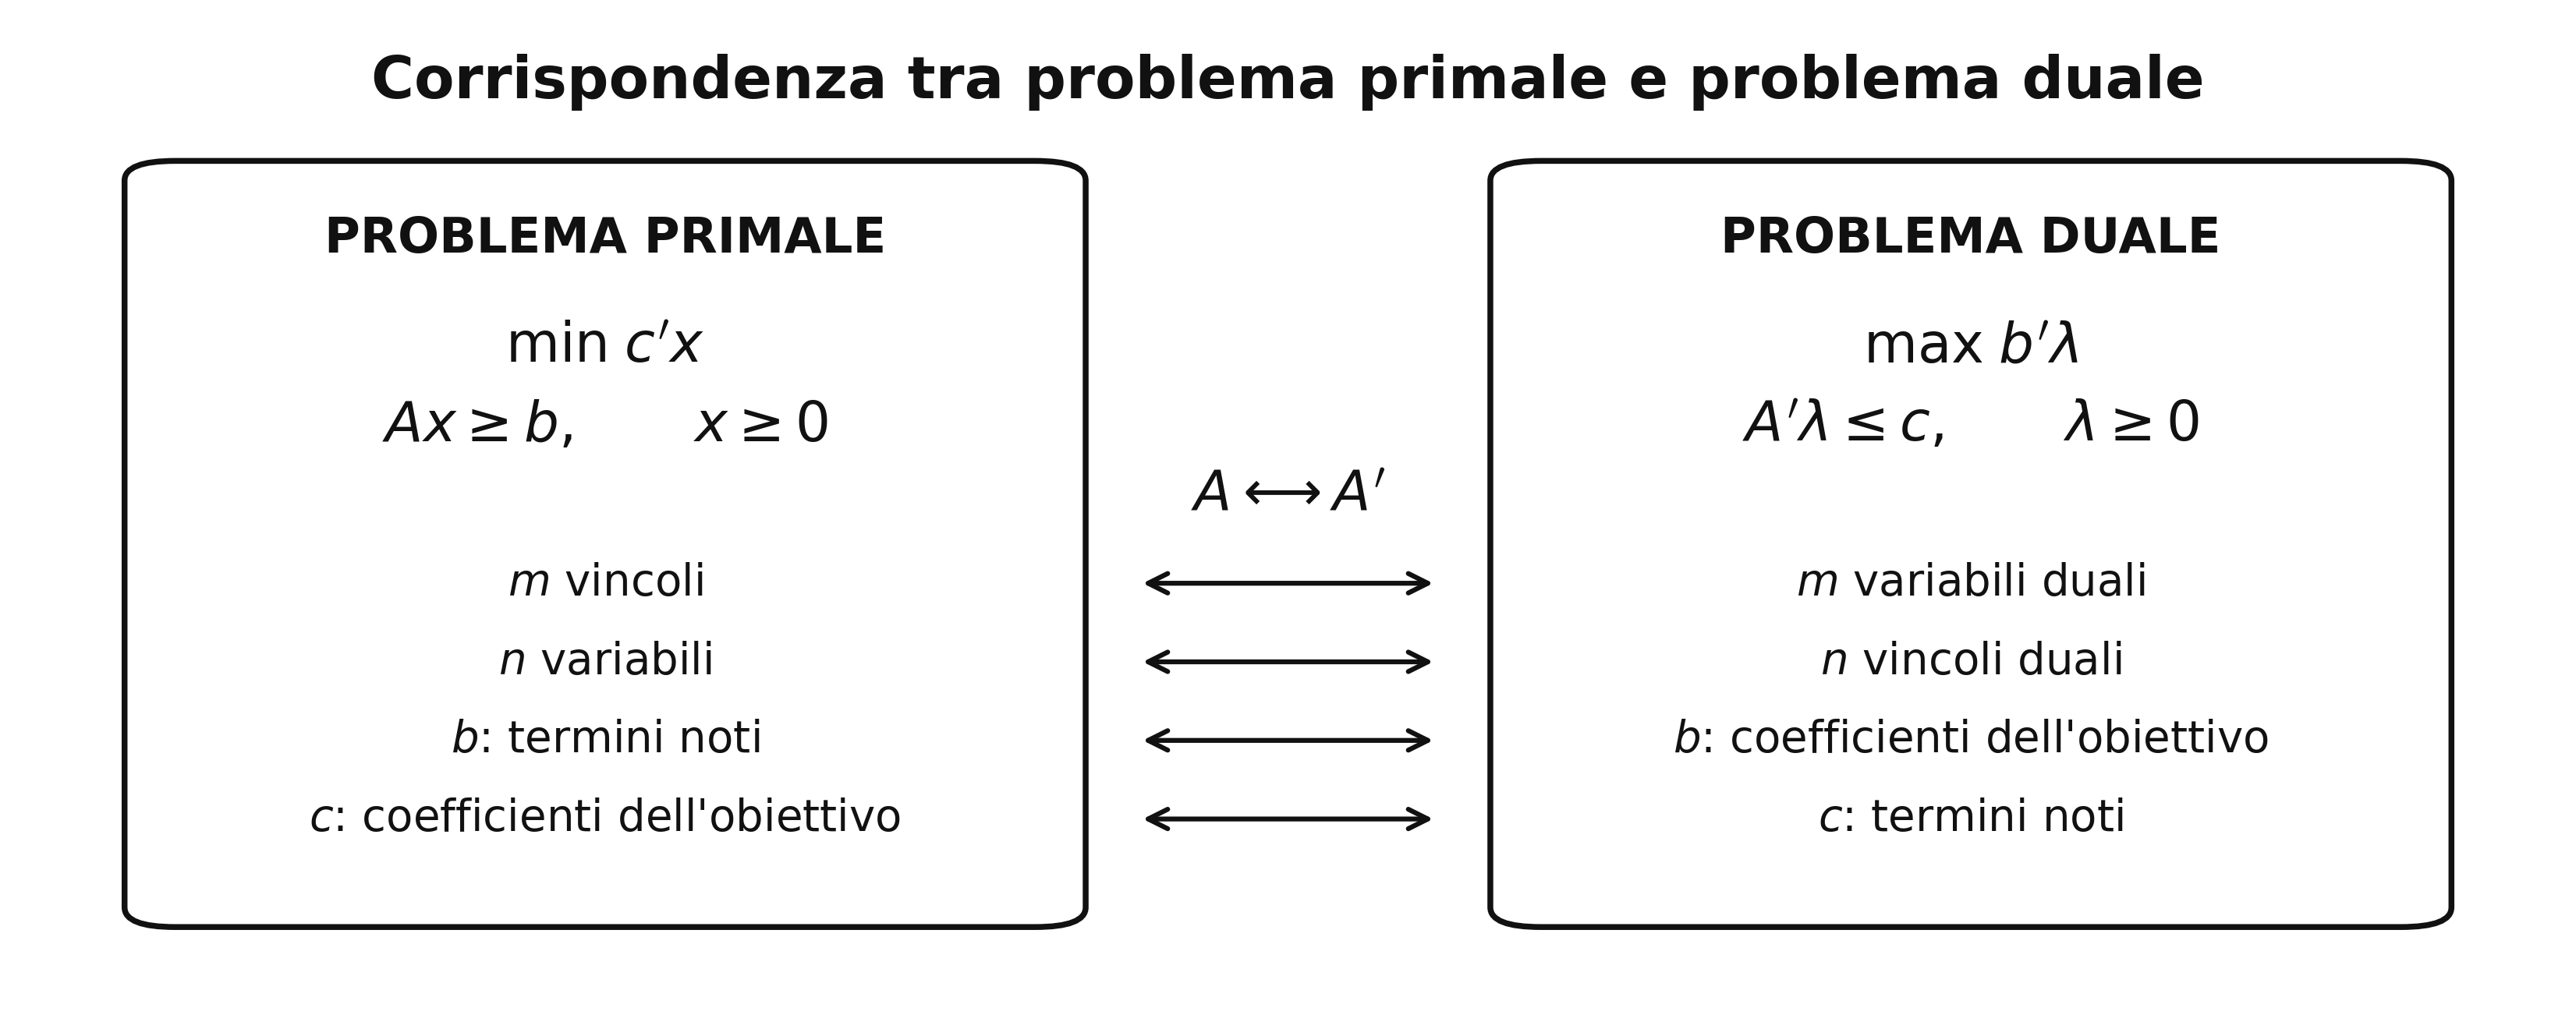
\includegraphics[width=0.84\textwidth]
{../graphics/cap11_corrispondenza_primale_duale.png}
\end{center}
 
\vspace{-2mm}
 
\begin{stepitemize}
\item A ogni \textbf{vincolo} del primale corrisponde una \textbf{variabile}
duale; a ogni \textbf{variabile} del primale corrisponde un \textbf{vincolo}
duale.
 
\item Il vettore $b$ passa nella funzione obiettivo; il vettore $c$ passa nel
lato destro dei vincoli; la matrice $A$ diventa $A'$.
 
\item Un modello con $4$ variabili e $4$ vincoli produce quindi un duale con
$4$ variabili e $4$ vincoli: i prezzi $\lambda$ vengono determinati \textbf{congiuntamente}, in una
sola soluzione.
\end{stepitemize}
 
%TCIMACRO{\TeXButton{Transition: Box Out}{\transboxout}}%
%BeginExpansion
\transboxout%
%EndExpansion
%TCIMACRO{\TeXButton{EndFrame}{\end{frame}}}%
%BeginExpansion
\end{frame}%
%EndExpansion
 
%****************************************
 
\subsection{Il duale del modello SVB}%
 
%TCIMACRO{\TeXButton{BeginFrame}{\begin{frame}}}%
%BeginExpansion
\begin{frame}%
%EndExpansion
 
\QTR{frametitle}{Il duale del modello SVB stilizzato}
 
%TCIMACRO{\TeXButton{Transparency}{\setbeamercovered{transparent=20}}}%
%BeginExpansion
\setbeamercovered{transparent=20}%
%EndExpansion
 
Un prezzo, chiamato solitamente \textbf{prezzo ombra}, per ciascuno dei quattro vincoli:
 
\medskip
 
{\small
\[
\begin{array}{ll}
\lambda_0\in\R & \mbox{bilancio (uguaglianza: libera in segno)}\\[2pt]
\lambda_Q\geq0 & \mbox{requisito minimo di liquidit\`{a}}\\[2pt]
\lambda_K\geq0 & \mbox{limite alla perdita sotto stress}\\[2pt]
\lambda_C\geq0 & \mbox{limite di concentrazione}
\end{array}
\]
}
 
\medskip
 
{\small
\[
\begin{array}{ll}
\min
&
100\lambda_0-55\lambda_Q+7\lambda_K+30\lambda_C
\\[4pt]
\mbox{soggetto a}
&
\lambda_0-\lambda_Q\geq0.010,
\\[2pt]
&
\lambda_0-0.90\lambda_Q+0.02\lambda_K\geq0.025,
\\[2pt]
&
\lambda_0-0.50\lambda_Q+0.15\lambda_K+\lambda_C\geq0.040,
\\[2pt]
&
\lambda_0-0.20\lambda_Q+0.08\lambda_K\geq0.050.
\end{array}
\]
}
 
\medskip
 
{\footnotesize Il segno negativo di $\lambda_Q$ nell'obiettivo deriva dalla
riscrittura del requisito $q'x\geq55$ nella forma $-q'x\leq-55$.}
 
%TCIMACRO{\TeXButton{Transition: Box Out}{\transboxout}}%
%BeginExpansion
\transboxout%
%EndExpansion
%TCIMACRO{\TeXButton{EndFrame}{\end{frame}}}%
%BeginExpansion
\end{frame}%
%EndExpansion
 
%****************************************
 
\subsection{Leggere un vincolo duale}%
 
%TCIMACRO{\TeXButton{BeginFrame}{\begin{frame}}}%
%BeginExpansion
\begin{frame}%
%EndExpansion
 
\QTR{frametitle}{Un vincolo duale per ogni classe di attivo}
 
%TCIMACRO{\TeXButton{Transparency}{\setbeamercovered{transparent=20}}}%
%BeginExpansion
\setbeamercovered{transparent=20}%
%EndExpansion
 
I quattro vincoli duali corrispondono, nell'ordine, a
$x_1,x_2,x_3,x_4$. Prendiamo quello dei \textbf{titoli a breve scadenza}:
 
\medskip
 
{\small
\[
\underbrace{
\lambda_0-0.90\lambda_Q+0.02\lambda_K
}_{\mbox{\footnotesize valore implicito delle risorse impiegate}}
\;\geq\;
\underbrace{
0.025
}_{\mbox{\footnotesize contributo economico unitario}}
\]
}
 
\medskip
 
\begin{stepitemize}
\item Una unit\`{a} di $x_2$ assorbe una unit\`{a} di bilancio, produce
$0.90$ di liquidit\`{a} e consuma $0.02$ della capacit\`{a} di assorbire
perdite.
 
\item Il vincolo impone che quell'impiego di risorse \textbf{valga almeno
quanto rende}. Se valesse meno, converrebbe aumentare $x_2$: la soluzione non
sarebbe ottima.
 
\item La colonna $j$ del primale, che nel Capitolo~11 descriveva \emph{come
$x_j$ contribuisce ai requisiti}, diventa qui \emph{il conto economico
implicito della classe $j$}.
\end{stepitemize}
 
%TCIMACRO{\TeXButton{Transition: Box Out}{\transboxout}}%
%BeginExpansion
\transboxout%
%EndExpansion
%TCIMACRO{\TeXButton{EndFrame}{\end{frame}}}%
%BeginExpansion
\end{frame}%
%EndExpansion
 
%****************************************
 
\subsection{Dualit\`{a} forte}%
 
%TCIMACRO{\TeXButton{BeginFrame}{\begin{frame}}}%
%BeginExpansion
\begin{frame}%
%EndExpansion
 
\QTR{frametitle}{Dualit\`{a} forte: i due valori coincidono}
 
%TCIMACRO{\TeXButton{Transparency}{\setbeamercovered{transparent=20}}}%
%BeginExpansion
\setbeamercovered{transparent=20}%
%EndExpansion
 
\begin{block}{Teorema (dualit\`{a} forte)}
{\small Se il primale ammette soluzione ottima finita, anche il duale la
ammette e i due valori coincidono: $c'x^{*}=b'\lambda^{*}$.}
\end{block}
 
\medskip
 
Nel modello SVB la soluzione duale \`{e}
 
{\small
\[
\lambda_0^{*}\approx0.05642,
\quad
\lambda_Q^{*}\approx0.03507,
\quad
\lambda_K^{*}\approx0.00746,
\quad
\lambda_C^{*}=0.
\]
}
 
\begin{stepitemize}
\item Verifica:
{\small
\[
100(0.05642)-55(0.03507)+7(0.00746)
\approx
3.765
=
z^{*}.
\]
}
 
\item \textbf{Massimo risultato ottenibile $=$ minimo valore implicito delle
risorse.}
 
\item E $\lambda_Q^{*}\approx0.03507$ \`{e} \emph{lo stesso numero} ottenuto
ieri ricalcolando l'ottimo requisito per requisito. Qui arriva insieme a tutti
gli altri, da una sola soluzione.
\end{stepitemize}
 
%TCIMACRO{\TeXButton{Transition: Box Out}{\transboxout}}%
%BeginExpansion
\transboxout%
%EndExpansion
%TCIMACRO{\TeXButton{EndFrame}{\end{frame}}}%
%BeginExpansion
\end{frame}%
%EndExpansion
 
%****************************************
 
\subsection{Complementariet\`{a}}%
 
%TCIMACRO{\TeXButton{BeginFrame}{\begin{frame}}}%
%BeginExpansion
\begin{frame}%
%EndExpansion
 
\QTR{frametitle}{Complementariet\`{a}: quali vincoli stanno decidendo}
 
%TCIMACRO{\TeXButton{Transparency}{\setbeamercovered{transparent=20}}}%
%BeginExpansion
\setbeamercovered{transparent=20}%
%EndExpansion
 
Per ogni vincolo, all'ottimo:
$\lambda_i^{*}s_i^{*}=0$, dove $s_i^{*}=b_i-a_i'x^{*}$ \`{e} il margine.
 
\medskip
 
{\small
\[
\begin{array}{l|c|c|c}
\hline
\mbox{vincolo} & \mbox{margine }s_i^{*} & \mbox{stato} & \lambda_i^{*}\\
\hline
\mbox{liquidit\`{a}}      & 0     & \mbox{attivo}  & 0.03507\\
\mbox{perdita sotto stress} & 0   & \mbox{attivo}  & 0.00746\\
\mbox{concentrazione}     & 9.104 & \mbox{inattivo}& 0\\
\hline
\end{array}
\]
}
 
\medskip
 
\begin{stepitemize}
\item \textbf{O il vincolo \`{e} attivo, o il suo prezzo \`{e} nullo.} Mai
entrambe le cose diverse da zero.
 
\item Il limite di concentrazione conserva un margine di $9.104$: allentarlo
non migliorerebbe di nulla il risultato, perch\'{e} non sta condizionando la
decisione.
 
\item La complementariet\`{a} \`{e} quindi uno strumento \textbf{diagnostico}:
dice quali requisiti stanno davvero determinando la scelta.
\end{stepitemize}
 
%TCIMACRO{\TeXButton{Transition: Box Out}{\transboxout}}%
%BeginExpansion
\transboxout%
%EndExpansion
%TCIMACRO{\TeXButton{EndFrame}{\end{frame}}}%
%BeginExpansion
\end{frame}%
%EndExpansion

\section{Liquidit\`{a} aggregata e liquidit\`{a} temporale}

%****************************************

\subsection{Che cosa misura il coefficiente di liquidabilit\`{a}}%

%TCIMACRO{\TeXButton{BeginFrame}{\begin{frame}}}%
%BeginExpansion
\begin{frame}%
%EndExpansion

\QTR{frametitle}{Il requisito aggregato comprime il tempo}

%TCIMACRO{\TeXButton{Transparency}{\setbeamercovered{transparent=20}}}%
%BeginExpansion
\setbeamercovered{transparent=20}%
%EndExpansion

Nella soluzione del Capitolo~11 il requisito di liquidit\`{a} \`{e} attivo:

{\small
\[
\sum_{j=1}^{4}q_jx_j^{*}
=
Q_{\min}
=
55.
\]
}

\medskip

\begin{stepitemize}
\item Il coefficiente $q_2=0.90$ dice che ogni unit\`{a} investita in titoli a
breve contribuisce per $0.90$ alla liquidit\`{a} disponibile.

\item Ma \textbf{disponibile quando?} Fra un mese, fra un anno, alla
scadenza del titolo? Il modello non lo dice.

\item Un solo numero per classe di attivo riassume l'intero profilo
temporale. La domanda \`{e} se questa compressione sia innocua.
\end{stepitemize}

%TCIMACRO{\TeXButton{Transition: Box Out}{\transboxout}}%
%BeginExpansion
\transboxout%
%EndExpansion
%TCIMACRO{\TeXButton{EndFrame}{\end{frame}}}%
%BeginExpansion
\end{frame}%
%EndExpansion

%****************************************

\subsection{Due portafogli, stesso totale}%

%TCIMACRO{\TeXButton{BeginFrame}{\begin{frame}}}%
%BeginExpansion
\begin{frame}%
%EndExpansion

\QTR{frametitle}{Due portafogli con lo stesso cash flow complessivo}

%TCIMACRO{\TeXButton{Transparency}{\setbeamercovered{transparent=20}}}%
%BeginExpansion
\setbeamercovered{transparent=20}%
%EndExpansion

Tre date, e due portafogli che producono in totale la stessa liquidit\`{a}:
\vspace{-2mm}

{\small
\[
A:\;(6,\;2,\;2),
\qquad
B:\;(1,\;2,\;7),
\qquad
\mbox{totale}=10\ \mbox{in entrambi i casi.}
\]
}

\vspace{-2mm}

\begin{center}
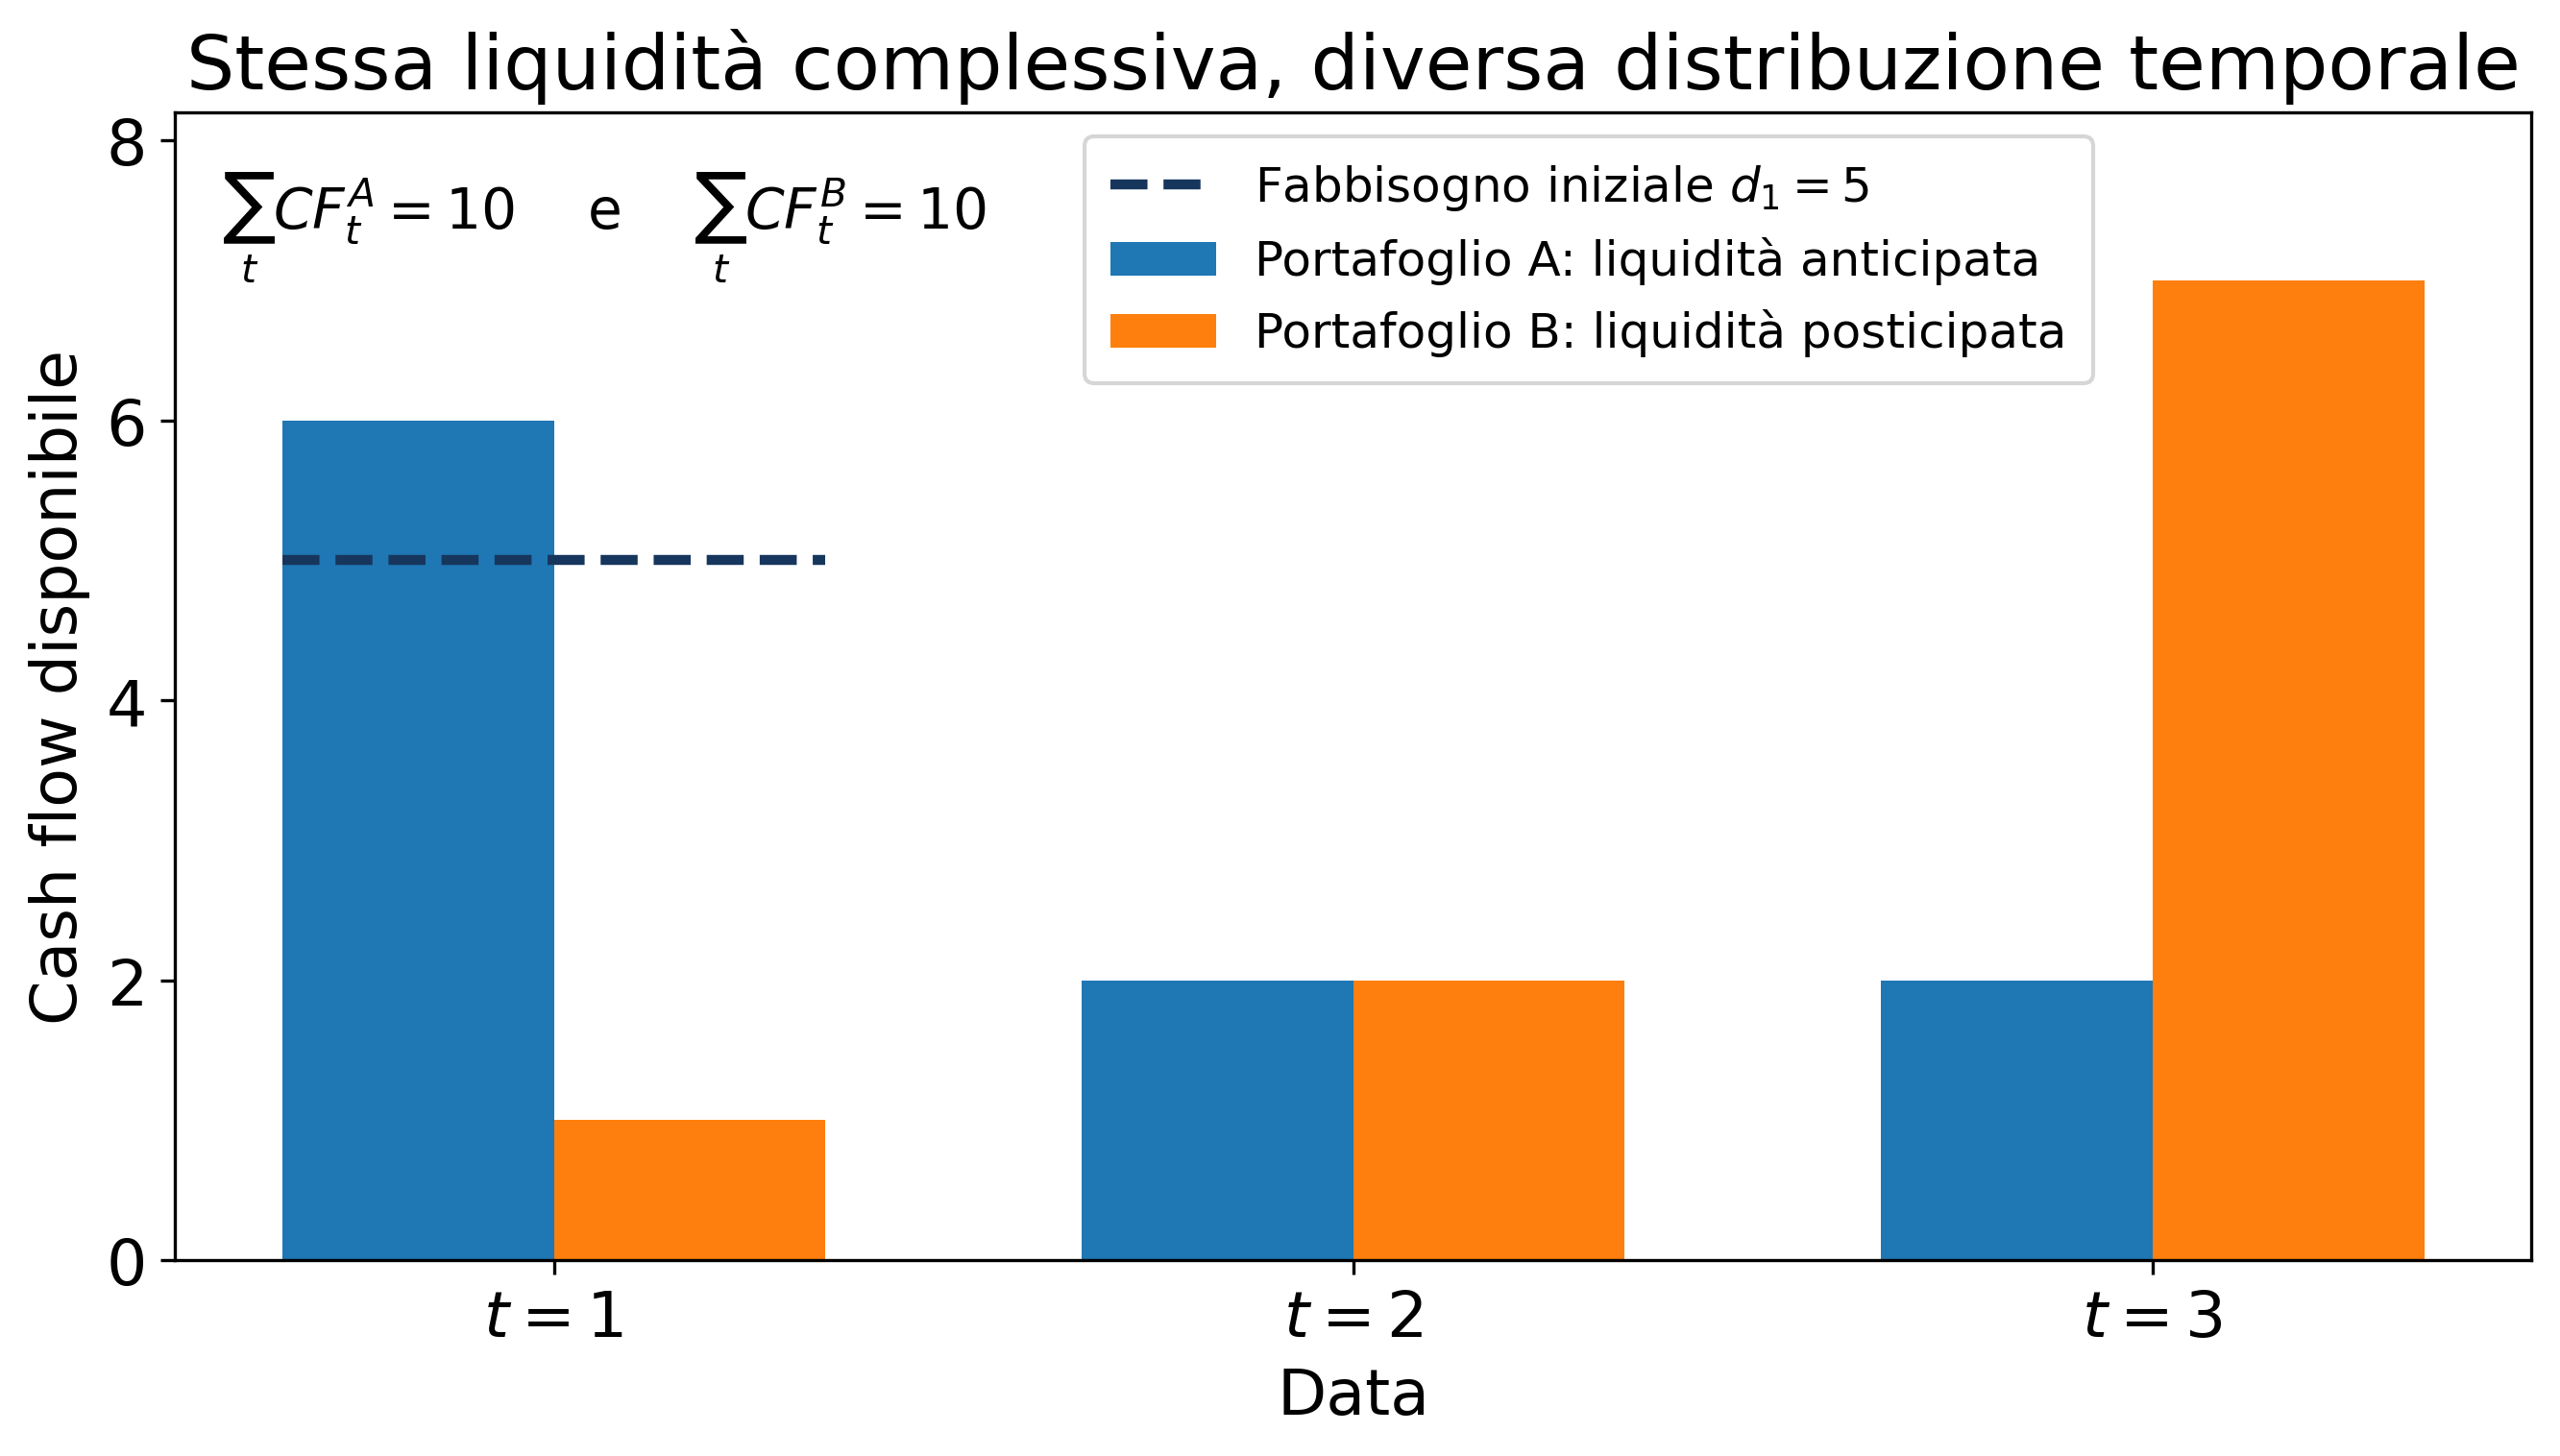
\includegraphics[width=0.78\textwidth]
{../graphics/Cap12_liquidita_aggregata_temporale.png}
\end{center}

\vspace{-2mm}

\begin{stepitemize}
\item Alla prima data la banca deve pagare $d_1=5$. Il portafoglio $A$
produce $6$: sufficiente. Il portafoglio $B$ produce $1$.

\end{stepitemize}

%TCIMACRO{\TeXButton{Transition: Box Out}{\transboxout}}%
%BeginExpansion
\transboxout%
%EndExpansion
%TCIMACRO{\TeXButton{EndFrame}{\end{frame}}}%
%BeginExpansion
\end{frame}%
%EndExpansion

%****************************************

\subsection{Dal requisito ai bilanci per data}%

%TCIMACRO{\TeXButton{BeginFrame}{\begin{frame}}}%
%BeginExpansion
\begin{frame}%
%EndExpansion

\QTR{frametitle}{Dal requisito aggregato ai bilanci per data}

%TCIMACRO{\TeXButton{Transparency}{\setbeamercovered{transparent=20}}}%
%BeginExpansion
\setbeamercovered{transparent=20}%
%EndExpansion

Lo stesso vale dal lato del passivo: la banca non fronteggia un unico
fabbisogno complessivo, ma una \textbf{successione} di rimborsi e deflussi
collocati in date diverse.

\medskip

Introduciamo quindi le date

{\small
\[
t=0,1,\ldots,T,
\]
}

dove $t=0$ \`{e} il momento in cui si sceglie la composizione del bilancio e
$t=1,\ldots,T$ sono le scadenze future.

{\small
\[
\boxed{
\mbox{requisito aggregato di liquidit\`{a}}
\quad\longrightarrow\quad
\mbox{bilanci di liquidit\`{a} alle diverse date}
}
\]
}

\begin{stepitemize}
\item \`{E} il punto di ingresso nell'\textbf{Asset--Liability Management}.

\item Il problema resta un \textbf{programma lineare}: non serve una nuova
tecnica di ottimizzazione. Cambiano i dati e la struttura dei vincoli.
\end{stepitemize}

%TCIMACRO{\TeXButton{Transition: Box Out}{\transboxout}}%
%BeginExpansion
\transboxout%
%EndExpansion
%TCIMACRO{\TeXButton{EndFrame}{\end{frame}}}%
%BeginExpansion
\end{frame}%
%EndExpansion

\section{La matrice dei cash flow}

%****************************************

\subsection{Il profilo temporale degli attivi}%

%TCIMACRO{\TeXButton{BeginFrame}{\begin{frame}}}%
%BeginExpansion
\begin{frame}%
%EndExpansion

\QTR{frametitle}{Un coefficiente per ogni classe e per ogni data}

%TCIMACRO{\TeXButton{Transparency}{\setbeamercovered{transparent=20}}}%
%BeginExpansion
\setbeamercovered{transparent=20}%
%EndExpansion

Al posto del singolo $q_j$, indichiamo con $a_{tj}$ il cash flow disponibile
alla data $t$ per una unit\`{a} investita nella classe $j$ al tempo $0$:

{\small
\[
A^{\mathrm{CF}}
=
\begin{pmatrix}
a_{11} & a_{12} & \cdots & a_{1n}\\
a_{21} & a_{22} & \cdots & a_{2n}\\
\vdots & \vdots & \ddots & \vdots\\
a_{T1} & a_{T2} & \cdots & a_{Tn}
\end{pmatrix},
\qquad
T\ \mbox{righe},\quad n\ \mbox{colonne}.
\]
}

\medskip

\begin{stepitemize}
\item Una \textbf{colonna} descrive il profilo temporale di una classe di
attivo: quando restituisce liquidit\`{a}.

\item Una \textbf{riga} descrive che cosa incassa la banca a una certa data
dalle diverse classi.

\item Il cash flow complessivo prodotto alla data $t$ \`{e}
$\sum_j a_{tj}x_j$, cio\`{e} la componente $t$-esima del vettore risultante da:
$$
A^{\mathrm{CF}}x
$$.
\end{stepitemize}

%TCIMACRO{\TeXButton{Transition: Box Out}{\transboxout}}%
%BeginExpansion
\transboxout%
%EndExpansion
%TCIMACRO{\TeXButton{EndFrame}{\end{frame}}}%
%BeginExpansion
\end{frame}%
%EndExpansion

%****************************************

\subsection{I fabbisogni alle diverse date}%

%TCIMACRO{\TeXButton{BeginFrame}{\begin{frame}}}%
%BeginExpansion
\begin{frame}%
%EndExpansion

\QTR{frametitle}{Risorse e fabbisogni, data per data}

%TCIMACRO{\TeXButton{Transparency}{\setbeamercovered{transparent=20}}}%
%BeginExpansion
\setbeamercovered{transparent=20}%
%EndExpansion

Dal lato del passivo, $d_t\geq0$ \`{e} il fabbisogno monetario da soddisfare
alla data $t$: rimborsi, pagamenti contrattuali, deflussi della raccolta.

\medskip

\begin{center}
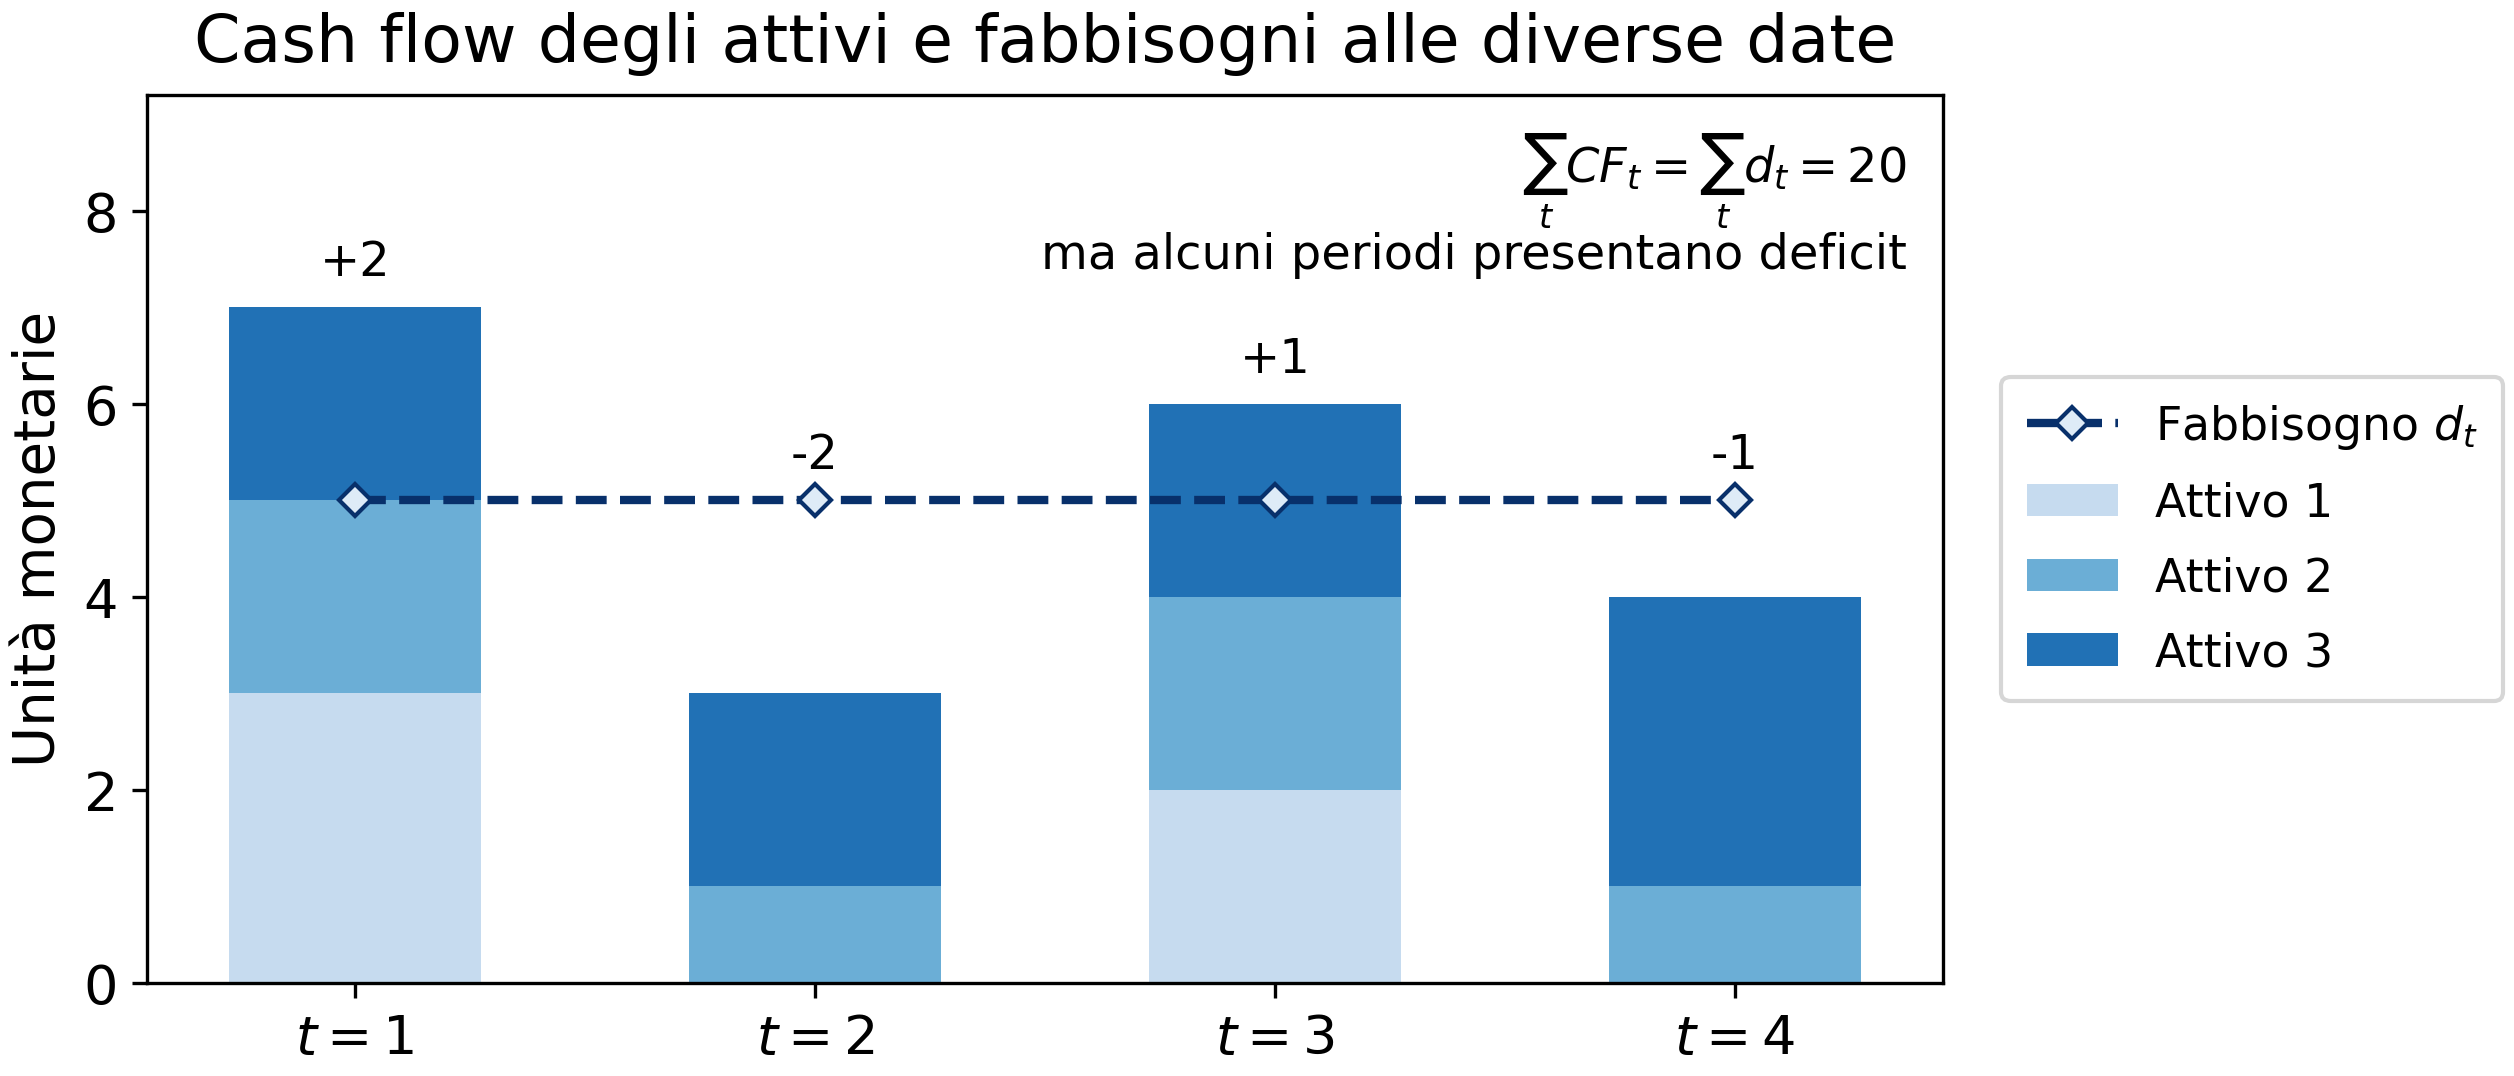
\includegraphics[width=0.80\textwidth]
{../graphics/Cap12_cashflow_attivi_fabbisogni_b.png}
\end{center}

\vspace{-2mm}

\begin{stepitemize}
\item Sull'intero orizzonte le risorse coincidono con i fabbisogni:
$\sum_t CF_t=\sum_t d_t$.

\item Eppure risultano \textbf{surplus} alle date $1$ e $3$ e
\textbf{deficit} alle date $2$ e $4$.

\item Il pareggio complessivo non garantisce la solvibilit\`{a} alle singole
scadenze.
\end{stepitemize}

%TCIMACRO{\TeXButton{Transition: Box Out}{\transboxout}}%
%BeginExpansion
\transboxout%
%EndExpansion
%TCIMACRO{\TeXButton{EndFrame}{\end{frame}}}%
%BeginExpansion
\end{frame}%
%EndExpansion

%****************************************

\subsection{Il cash-flow matching}%

%TCIMACRO{\TeXButton{BeginFrame}{\begin{frame}}}%
%BeginExpansion
\begin{frame}%
%EndExpansion

\QTR{frametitle}{Una prima formulazione: cash-flow matching}

%TCIMACRO{\TeXButton{Transparency}{\setbeamercovered{transparent=20}}}%
%BeginExpansion
\setbeamercovered{transparent=20}%
%EndExpansion

Richiediamo che a \emph{ciascuna} data i cash flow prodotti bastino a coprire
il fabbisogno:

{\small
\[
\sum_{j=1}^{n}a_{tj}x_j
\;\geq\;
d_t,
\qquad
t=1,\ldots,T,
\qquad\mbox{ovvero}\qquad
A^{\mathrm{CF}}x\geq d.
\]
}

\medskip

{\small
\[
\underbrace{
\sum_{j=1}^{n}q_jx_j\geq Q_{\min}
}_{\mbox{\footnotesize un requisito complessivo}}
\qquad\longrightarrow\qquad
\underbrace{
A^{\mathrm{CF}}x\geq d
}_{\mbox{\footnotesize $T$ requisiti datati}}
\]
}

\medskip

\begin{stepitemize}
\item Nel primo caso la liquidit\`{a} \`{e} una \textbf{caratteristica} della
composizione dell'attivo.

\item Nel secondo \`{e} confrontata con obblighi che hanno una
\textbf{scadenza precisa}.
\end{stepitemize}

%TCIMACRO{\TeXButton{Transition: Box Out}{\transboxout}}%
%BeginExpansion
\transboxout%
%EndExpansion
%TCIMACRO{\TeXButton{EndFrame}{\end{frame}}}%
%BeginExpansion
\end{frame}%
%EndExpansion

%****************************************

\subsection{Il limite del matching separato}%

%TCIMACRO{\TeXButton{BeginFrame}{\begin{frame}}}%
%BeginExpansion
\begin{frame}%
%EndExpansion

\QTR{frametitle}{Perch\'{e} ancora non basta: le date restano scollegate}

%TCIMACRO{\TeXButton{Transparency}{\setbeamercovered{transparent=20}}}%
%BeginExpansion
\setbeamercovered{transparent=20}%
%EndExpansion

Supponiamo che alla data $t$ il portafoglio produca pi\`{u} del necessario:

{\small
\[
\sum_{j=1}^{n}a_{tj}x_j-d_t
\;>\;
0.
\]
}

\medskip

\begin{stepitemize}
\item Quell'eccedenza \textbf{non viene utilizzata} nel vincolo della data $t+1$: nel
modello semplicemente svanisce.

\item Ma una banca la conserva, o la reinveste. La posizione di liquidit\`{a}
di una data dipende da che cosa \`{e} accaduto nelle date precedenti.

\item I $T$ vincoli non sono quindi indipendenti: serve una variabile che
\textbf{trasporti} la liquidit\`{a} da un periodo al successivo.
\end{stepitemize}

\medskip

{\small
\[
\boxed{
\mbox{cash-flow matching per data}
\quad\longrightarrow\quad
\mbox{bilanci collegati nel tempo}
}
\]
}

%TCIMACRO{\TeXButton{Transition: Box Out}{\transboxout}}%
%BeginExpansion
\transboxout%
%EndExpansion
%TCIMACRO{\TeXButton{EndFrame}{\end{frame}}}%
%BeginExpansion
\end{frame}%
%EndExpansion

\section{Giacenze e bilanci intertemporali}

%****************************************

\subsection{La giacenza di liquidita}%

%TCIMACRO{\TeXButton{BeginFrame}{\begin{frame}}}%
%BeginExpansion
\begin{frame}%
%EndExpansion

\QTR{frametitle}{La variabile che trasporta la liquidit\`{a}}

%TCIMACRO{\TeXButton{Transparency}{\setbeamercovered{transparent=20}}}%
%BeginExpansion
\setbeamercovered{transparent=20}%
%EndExpansion

\begin{block}{Giacenza di liquidit\`{a}}
{\small Per ogni data $t=1,\ldots,T$, indichiamo con $g_t\geq0$ la
liquidit\`{a} che rimane disponibile \emph{immediatamente dopo} avere
soddisfatto il fabbisogno $d_t$.}
\end{block}

\medskip

\begin{stepitemize}
\item $g_t$ \`{e} uno \textbf{stock}, non un flusso: non \`{e} liquidit\`{a}
prodotta dall'attivo, ma quella che l'attivo ha prodotto e la banca non ha
speso.

\item \`{E} una \textbf{variabile decisionale} come $x_j$, ma di natura
diversa: le $x_j$ si scelgono al tempo $0$, le $g_t$ descrivono la posizione
con cui la banca esce da ciascuna data.

\item La condizione $g_t\geq0$ non \`{e} un dettaglio tecnico: \textbf{\`{e}
la condizione di solvibilit\`{a}} alla data $t$.
\end{stepitemize}

%TCIMACRO{\TeXButton{Transition: Box Out}{\transboxout}}%
%BeginExpansion
\transboxout%
%EndExpansion
%TCIMACRO{\TeXButton{EndFrame}{\end{frame}}}%
%BeginExpansion
\end{frame}%
%EndExpansion

%****************************************

\subsection{Il primo bilancio e il collegamento}%

%TCIMACRO{\TeXButton{BeginFrame}{\begin{frame}}}%
%BeginExpansion
\begin{frame}%
%EndExpansion

\QTR{frametitle}{Dalla disuguaglianza all'uguaglianza}

%TCIMACRO{\TeXButton{Transparency}{\setbeamercovered{transparent=20}}}%
%BeginExpansion
\setbeamercovered{transparent=20}%
%EndExpansion

Alla prima data, tutte le risorse disponibili devono avere una destinazione:

{\small
\[
\sum_{j=1}^{n}a_{1j}x_j
\;=\;
\underbrace{d_1}_{\mbox{\footnotesize speso}}
+
\underbrace{g_1}_{\mbox{\footnotesize conservato}}
\]
}

\medskip

\begin{stepitemize}
\item \`{E} un'\textbf{uguaglianza}, non pi\`{u} una disuguaglianza: nulla
svanisce.

\item Alla data $2$ la banca dispone dei nuovi cash flow \emph{e} di
$g_1$:

{\small
\[
\sum_{j=1}^{n}a_{2j}x_j+g_1=d_2+g_2.
\]
}

\item La stessa $g_1$ compare in \textbf{due bilanci consecutivi}: come
destinazione nel primo, come risorsa nel secondo.
\end{stepitemize}

\medskip

{\small
\[
\boxed{
g_t\ \mbox{collega il bilancio della data }t\mbox{ a quello della data }t+1
}
\]
}

%TCIMACRO{\TeXButton{Transition: Box Out}{\transboxout}}%
%BeginExpansion
\transboxout%
%EndExpansion
%TCIMACRO{\TeXButton{EndFrame}{\end{frame}}}%
%BeginExpansion
\end{frame}%
%EndExpansion

%****************************************

\subsection{Il sistema dei bilanci temporali}%

%TCIMACRO{\TeXButton{BeginFrame}{\begin{frame}}}%
%BeginExpansion
\begin{frame}%
%EndExpansion

\QTR{frametitle}{Il sistema completo, con il rendimento della giacenza}

%TCIMACRO{\TeXButton{Transparency}{\setbeamercovered{transparent=20}}}%
%BeginExpansion
\setbeamercovered{transparent=20}%
%EndExpansion

La liquidit\`{a} trasferita non resta ferma: impiegata fino alla data
successiva al tasso $r_{t-1}^{g}$, una unit\`{a} ne diventa
$1+r_{t-1}^{g}$.

\medskip

{\small
\[
\begin{array}{rcl}
\displaystyle\sum_{j=1}^{n}a_{1j}x_j-g_1
&=&
d_1,
\\[8pt]
\displaystyle\sum_{j=1}^{n}a_{2j}x_j+(1+r_1^{g})g_1-g_2
&=&
d_2,
\\
&\vdots&
\\
\displaystyle\sum_{j=1}^{n}a_{Tj}x_j+(1+r_{T-1}^{g})g_{T-1}-g_T
&=&
d_T.
\end{array}
\]
}

\medskip

\begin{stepitemize}
\item Il coefficiente $1+r_{t-1}^{g}$ \textbf{non altera la linearit\`{a}}:
$r_{t-1}^{g}$ \`{e} un dato, non una variabile.

\item Ogni $g_t$ compare in due righe consecutive, con segno opposto: \`{e}
la struttura a scala tipica dei modelli ALM.
\end{stepitemize}

%TCIMACRO{\TeXButton{Transition: Box Out}{\transboxout}}%
%BeginExpansion
\transboxout%
%EndExpansion
%TCIMACRO{\TeXButton{EndFrame}{\end{frame}}}%
%BeginExpansion
\end{frame}%
%EndExpansion

%****************************************

\subsection{Variabile di stato e condizione terminale}%

%TCIMACRO{\TeXButton{BeginFrame}{\begin{frame}}}%
%BeginExpansion
\begin{frame}%
%EndExpansion

\QTR{frametitle}{La liquidit\`{a} come variabile di stato}

%TCIMACRO{\TeXButton{Transparency}{\setbeamercovered{transparent=20}}}%
%BeginExpansion
\setbeamercovered{transparent=20}%
%EndExpansion

Dal bilancio segue una relazione ricorsiva, con $g_0=0$:

{\small
\[
g_t
=
g_{t-1}
+
\sum_{j=1}^{n}a_{tj}x_j
-
d_t,
\qquad
t=1,\ldots,T.
\]
}

\medskip

{\small
\[
\boxed{
\begin{array}{c}
\mbox{la posizione finanziaria a una data dipende anche}\\
\mbox{dalle decisioni e dai saldi accumulati in precedenza}
\end{array}
}
\]
}

\medskip

\begin{stepitemize}
\item \textbf{Condizione terminale.} Se all'orizzonte tutti gli obblighi sono
esauriti e alla liquidit\`{a} residua non si attribuisce valore, si pu\`{o}
imporre $g_T=0$.

\item Se invece $g_T$ resta libera, la banca pu\`{o} concludere l'orizzonte
con un margine. \textbf{Ce ne ricorderemo}: sar\`{a} la ragione per cui, nel
caso SVB, la liquidit\`{a} dell'ultima data avr\`{a} prezzo nullo.
\end{stepitemize}

%TCIMACRO{\TeXButton{Transition: Box Out}{\transboxout}}%
%BeginExpansion
\transboxout%
%EndExpansion
%TCIMACRO{\TeXButton{EndFrame}{\end{frame}}}%
%BeginExpansion
\end{frame}%
%EndExpansion

\section{Funding e obblighi di rimborso}

%****************************************

\subsection{Una fonte di funding a un periodo}%

%TCIMACRO{\TeXButton{BeginFrame}{\begin{frame}}}%
%BeginExpansion
\begin{frame}%
%EndExpansion

\QTR{frametitle}{Quando le risorse interne non bastano}

%TCIMACRO{\TeXButton{Transparency}{\setbeamercovered{transparent=20}}}%
%BeginExpansion
\setbeamercovered{transparent=20}%
%EndExpansion

Finora la banca dispone solo di ci\`{o} che l'attivo produce e di ci\`{o} che
ha conservato. Se non basta, pu\`{o} rivolgersi all'esterno.

\medskip

Indichiamo con $u_t\geq0$ il funding raccolto alla data $t$, per
$t=1,\ldots,T-1$, rimborsabile alla data successiva al tasso $r_t^{u}$.

\medskip

{\small
\[
\boxed{
\begin{array}{c}
\mbox{funding raccolto alla data }t:\quad u_t\\[3pt]
\downarrow\\[3pt]
\mbox{liquidit\`{a} disponibile alla data }t\\[3pt]
\downarrow\\[3pt]
\mbox{rimborso alla data }t+1:\quad (1+r_t^{u})u_t
\end{array}
}
\]
}

\medskip

\begin{stepitemize}
\item Il funding \textbf{non crea risorse}: le sposta nel tempo, dal futuro
al presente.

\item Alla data finale non si raccoglie nuovo funding: un prestito acceso in
$T$ andrebbe rimborsato oltre l'orizzonte del modello.
\end{stepitemize}

%TCIMACRO{\TeXButton{Transition: Box Out}{\transboxout}}%
%BeginExpansion
\transboxout%
%EndExpansion
%TCIMACRO{\TeXButton{EndFrame}{\end{frame}}}%
%BeginExpansion
\end{frame}%
%EndExpansion

%****************************************

\subsection{Il bilancio completo}%

%TCIMACRO{\TeXButton{BeginFrame}{\begin{frame}}}%
%BeginExpansion
\begin{frame}%
%EndExpansion

\QTR{frametitle}{Il bilancio di liquidit\`{a} in forma completa}

%TCIMACRO{\TeXButton{Transparency}{\setbeamercovered{transparent=20}}}%
%BeginExpansion
\setbeamercovered{transparent=20}%
%EndExpansion

Alla generica data intermedia, tre risorse e tre impieghi:

{\small
\[
\underbrace{
\sum_{j=1}^{n}a_{tj}x_j
+
(1+r_{t-1}^{g})g_{t-1}
+
u_t
}_{\mbox{\footnotesize cash flow, giacenza ereditata, nuovo funding}}
\;=\;
\underbrace{
d_t
+
(1+r_{t-1}^{u})u_{t-1}
+
g_t
}_{\mbox{\footnotesize fabbisogno, rimborso, giacenza trasferita}}
\]
}

\medskip

\begin{center}
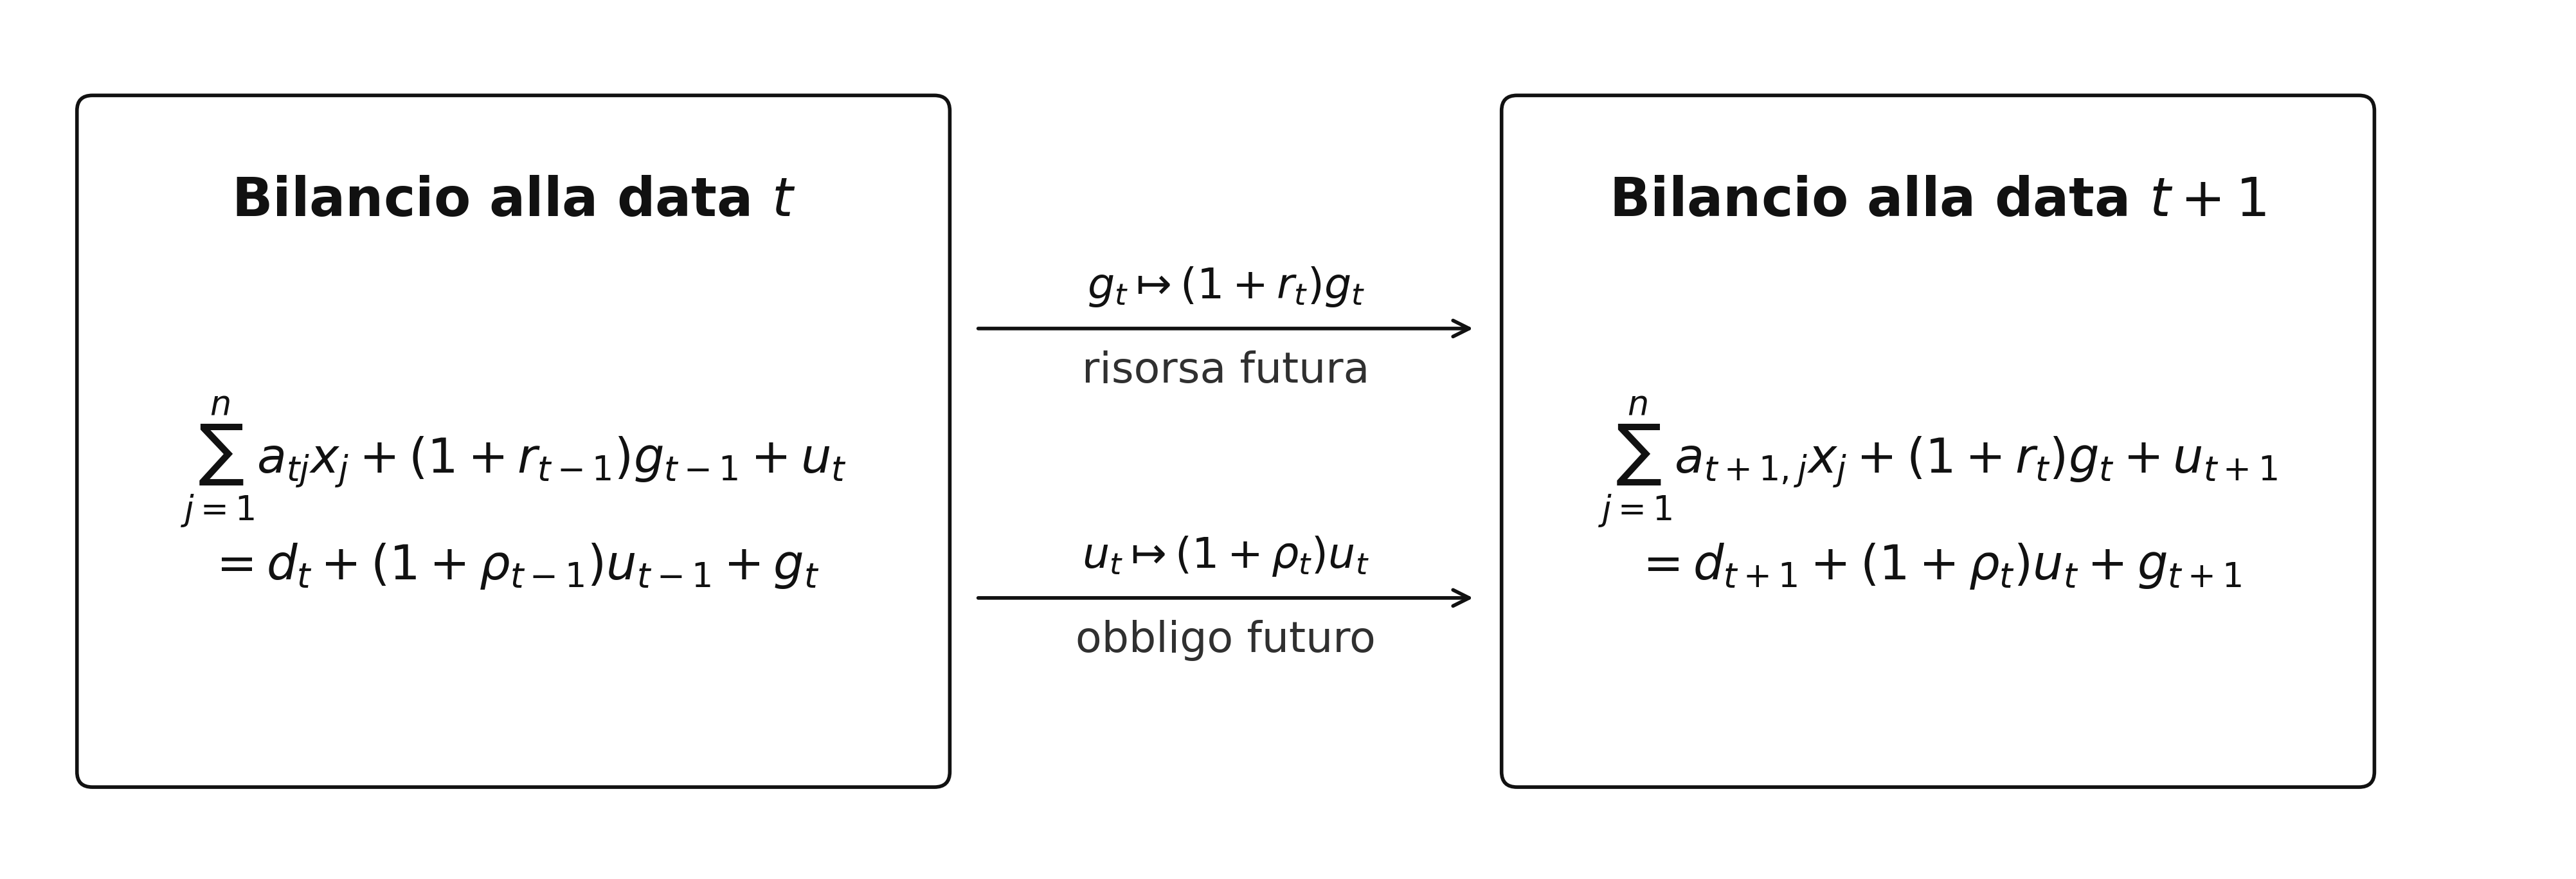
\includegraphics[width=0.84\textwidth]
{../graphics/Cap12_bilancio_intertemporale.png}
\end{center}

%TCIMACRO{\TeXButton{Transition: Box Out}{\transboxout}}%
%BeginExpansion
\transboxout%
%EndExpansion
%TCIMACRO{\TeXButton{EndFrame}{\end{frame}}}%
%BeginExpansion
\end{frame}%
%EndExpansion

%****************************************

\subsection{Due collegamenti di segno opposto}%

%TCIMACRO{\TeXButton{BeginFrame}{\begin{frame}}}%
%BeginExpansion
\begin{frame}%
%EndExpansion

\QTR{frametitle}{Due modi di attraversare il tempo}

%TCIMACRO{\TeXButton{Transparency}{\setbeamercovered{transparent=20}}}%
%BeginExpansion
\setbeamercovered{transparent=20}%
%EndExpansion

{\small
\[
\begin{array}{l|c|c}
\hline
 & \mbox{giacenza }g_t & \mbox{funding }u_t\\
\hline
\mbox{alla data }t   & \mbox{impiego} & \mbox{risorsa}\\
\mbox{alla data }t+1 & \mbox{risorsa} & \mbox{impiego}\\
\mbox{direzione}     & \mbox{presente}\rightarrow\mbox{futuro}
                     & \mbox{futuro}\rightarrow\mbox{presente}\\
\mbox{costo}         & \mbox{rende }r_t^{g} & \mbox{costa }r_t^{u}\\
\hline
\end{array}
\]
}

\medskip

\begin{stepitemize}
\item La giacenza \textbf{accumula} una risorsa per il periodo successivo; il
funding \textbf{anticipa} una risorsa creando un'obbligazione futura.

\item Il funding non elimina il problema di liquidit\`{a}: ne
\textbf{ridistribuisce} la collocazione temporale.

\item Coprire un deficit alla data $t$ pu\`{o} rendere pi\`{u} difficile il
bilancio alla data $t+1$, per via del rimborso $(1+r_t^{u})u_t$.
\end{stepitemize}

%TCIMACRO{\TeXButton{Transition: Box Out}{\transboxout}}%
%BeginExpansion
\transboxout%
%EndExpansion
%TCIMACRO{\TeXButton{EndFrame}{\end{frame}}}%
%BeginExpansion
\end{frame}%
%EndExpansion

%****************************************

\subsection{Capacita e costo del funding}%

%TCIMACRO{\TeXButton{BeginFrame}{\begin{frame}}}%
%BeginExpansion
\begin{frame}%
%EndExpansion

\QTR{frametitle}{Quanto funding, e a quale costo}

%TCIMACRO{\TeXButton{Transparency}{\setbeamercovered{transparent=20}}}%
%BeginExpansion
\setbeamercovered{transparent=20}%
%EndExpansion

La raccolta esterna non \`{e} illimitata:

{\small
\[
0\leq u_t\leq\bar u_t,
\qquad
t=1,\ldots,T-1.
\]
}

Il limite $\bar u_t$ pu\`{o} riflettere linee di credito, accesso al mercato,
vincoli contrattuali. Attenzione a non confonderlo con $u_t$: il primo \`{e}
la \textbf{capacit\`{a}}, il secondo la \textbf{decisione}.

\medskip

\begin{stepitemize}
\item Assumiamo inoltre

{\small
\[
r_t^{u}\;\geq\;r_t^{g}.
\]
}

\item Senza questa condizione il modello raccoglierebbe funding \emph{solo}
per parcheggiarlo come giacenza e lucrare la differenza: un arbitraggio
artificiale, prodotto dalla formulazione e non dal problema economico.

\item La differenza $r_t^{u}-r_t^{g}$ misura, in forma stilizzata, il costo
di accedere alla raccolta esterna.
\end{stepitemize}

%TCIMACRO{\TeXButton{Transition: Box Out}{\transboxout}}%
%BeginExpansion
\transboxout%
%EndExpansion
%TCIMACRO{\TeXButton{EndFrame}{\end{frame}}}%
%BeginExpansion
\end{frame}%
%EndExpansion

%****************************************
\section{Il modello ALM deterministico}

\subsection{Ambiente, stato, solidita}%

%TCIMACRO{\TeXButton{BeginFrame}{\begin{frame}}}%
%BeginExpansion
\begin{frame}%
%EndExpansion

\QTR{frametitle}{Ambiente, stato, solidit\`{a}: tre livelli distinti}

%TCIMACRO{\TeXButton{Transparency}{\setbeamercovered{transparent=20}}}%
%BeginExpansion
\setbeamercovered{transparent=20}%
%EndExpansion

I coefficienti $r_t^{g}$, $r_t^{u}$, $\bar u_t$, $d_t$ non cadono dal cielo.
Dipendono da tre aspetti:

{\small
\[
\begin{array}{l|l}
\hline
\bar Z_t & \mbox{vettore, \textbf{esterno}: tassi, spread, tensione sul funding}\\
X_t      & \mbox{vettore, \textbf{interno}: attivo, liquidit\`{a}, capitale, funding}\\
\kappa_t      & \mbox{scalare, \textbf{valutazione}: }\kappa_t=\kappa(X_t,\bar Z_t)\\
\hline
\end{array}
\]
}

\begin{stepitemize}
\item $\bar Z_t$ \`{e} il mercato: la banca lo subisce, non lo sceglie. $X_t$
\`{e} il bilancio con cui lo affronta.

\item $\kappa_t=\kappa(X_t,\bar Z_t)$ \`{e} una \textbf{funzione}: prende lo stato della banca (e.g. il bilancio) e le condizioni di mercato e restituisce un numero, la
capacit\`{a} di assorbire uno shock.

\item \`{E} la dipendenza da $X_t$ a contare: davanti allo \textbf{stesso}
$\bar Z_t$, due bilanci diversi danno solidit\`{a} diverse -- e quindi
deflussi diversi.

{\small
\[
\boxed{
\bar Z_t,\ X_t
\;\longrightarrow\;
\kappa_t
\;\longrightarrow\;
d_t
}
\]
}
\end{stepitemize}


%TCIMACRO{\TeXButton{Transition: Box Out}{\transboxout}}%
%BeginExpansion
\transboxout%
%EndExpansion
%TCIMACRO{\TeXButton{EndFrame}{\end{frame}}}%
%BeginExpansion
\end{frame}%
%EndExpansion

%****************************************

\subsection{La formulazione completa}%

%TCIMACRO{\TeXButton{BeginFrame}{\begin{frame}}}%
%BeginExpansion
\begin{frame}%
%EndExpansion

\QTR{frametitle}{Il programma lineare completo}

%TCIMACRO{\TeXButton{Transparency}{\setbeamercovered{transparent=20}}}%
%BeginExpansion
\setbeamercovered{transparent=20}%
%EndExpansion

{\footnotesize
\[
\begin{array}{ll}
\max\limits_{x,g,u}
&
\displaystyle
\sum_{j=1}^{n}c_jx_j
+
\sum_{t=1}^{T-1}r_t^{g}g_t
-
\sum_{t=1}^{T-1}r_t^{u}u_t
\qquad=\ \Pi(x,g,u)
\\[10pt]
\mbox{s.a}
&
\displaystyle\sum_{j=1}^{n}x_j=A_0
\\[8pt]
&
\displaystyle\sum_{j=1}^{n}a_{1j}x_j+u_1-g_1=d_1
\\[8pt]
&
\displaystyle\sum_{j=1}^{n}a_{tj}x_j+(1+r_{t-1}^{g})g_{t-1}+u_t
-(1+r_{t-1}^{u})u_{t-1}-g_t=d_t
\\[-2pt]
&
\hfill t=2,\ldots,T-1
\\[8pt]
&
\displaystyle\sum_{j=1}^{n}a_{Tj}x_j+(1+r_{T-1}^{g})g_{T-1}
-(1+r_{T-1}^{u})u_{T-1}-g_T=d_T
\\[8pt]
&
\ell'x\leq K,
\qquad
x_3\leq\alpha A_0
\\[4pt]
&
0\leq u_t\leq\bar u_t,
\qquad
g_t\geq0,
\qquad
x_j\geq0
\end{array}
\]
}

{\footnotesize $q'x\geq Q_{\min}$ \textbf{non compare pi\`{u}}: lo sostituiscono
i bilanci temporali. In questa fase vogliamo mantenere la linearit\`{a} del problema ALM, pertanto i deflussi $d_t$ \textbf{entrano come dato}, cioè non dipendono da $X_t$.}

%TCIMACRO{\TeXButton{Transition: Box Out}{\transboxout}}%
%BeginExpansion
\transboxout%
%EndExpansion
%TCIMACRO{\TeXButton{EndFrame}{\end{frame}}}%
%BeginExpansion
\end{frame}%
%EndExpansion


%****************************************

\subsection{Perche resta un programma lineare}%

%TCIMACRO{\TeXButton{BeginFrame}{\begin{frame}}}%
%BeginExpansion
\begin{frame}%
%EndExpansion

\QTR{frametitle}{Pi\`{u} date, stessa classe di problemi}

%TCIMACRO{\TeXButton{Transparency}{\setbeamercovered{transparent=20}}}%
%BeginExpansion
\setbeamercovered{transparent=20}%
%EndExpansion

\begin{stepitemize}
\item Le variabili $x_j$, $g_t$, $u_t$ compaiono tutte \textbf{al primo
grado}.

\item Anche $(1+r_{t-1}^{g})g_{t-1}$ e $(1+r_{t-1}^{u})u_{t-1}$ sono lineari:
i tassi sono coefficienti noti, non variabili.

\item La struttura temporale aumenta il \emph{numero} e l'\emph{organizzazione}
dei vincoli, non la difficolt\`{a} matematica.
\end{stepitemize}

\medskip

{\small
\[
\boxed{
\begin{array}{c}
\mbox{ALM deterministico}\\[3pt]
=\\[3pt]
\mbox{programma lineare con bilanci collegati nel tempo}
\end{array}
}
\]
}

\medskip

{\footnotesize Nella \textbf{Lezione 13} raccoglieremo $x$, $g$ e $u$ in un
unico vettore $v$, costruiremo $A_{\mathrm{eq}}$ e $A_{\mathrm{ub}}$ e
passeremo il problema a \texttt{scipy.optimize.linprog} con il metodo
\texttt{highs}. Oggi ci fermiamo alla formulazione e alla sua lettura
economica.}

%TCIMACRO{\TeXButton{Transition: Box Out}{\transboxout}}%
%BeginExpansion
\transboxout%
%EndExpansion
%TCIMACRO{\TeXButton{EndFrame}{\end{frame}}}%
%BeginExpansion
\end{frame}%
%EndExpansion

\section{Esercizio in aula: fattibilita temporale}

%****************************************

\subsection{La consegna}%

%TCIMACRO{\TeXButton{BeginFrame}{\begin{frame}}}%
%BeginExpansion
\begin{frame}%
%EndExpansion

\QTR{frametitle}{Esercizio: la composizione regge nel tempo?}

%TCIMACRO{\TeXButton{Transparency}{\setbeamercovered{transparent=20}}}%
%BeginExpansion
\setbeamercovered{transparent=20}%
%EndExpansion

Una banca ha investito $20$ in ciascuna di due classi di attivo. Tre date.

{\small
\[
A^{\mathrm{CF}}
=
\begin{pmatrix}
0.70 & 0.10\\
0.30 & 0.30\\
0    & 0.60
\end{pmatrix},
\qquad
x=\begin{pmatrix}20\\20\end{pmatrix},
\qquad
d'=(15,\;14,\;8).
\]
}

{\small
\[
r_1^{g}=0.005,
\qquad
u_1=0,
\qquad
r_2^{u}=0.020,
\qquad
\bar u_2=3.
\]
}

\medskip

\begin{stepenumerate}
\item [1.] Calcolare il profilo dei cash flow prodotti dall'attivo.

\item [2.] Verificare se i tre fabbisogni sono soddisfatti \textbf{senza}
ricorrere al funding.

\item [3.] Determinare il funding minimo necessario alla seconda data e la
giacenza terminale che ne risulta.

\item [4.] Che cosa accadrebbe se la capacit\`{a} scendesse a
$\bar u_2=0.8$?
\end{stepenumerate}

%TCIMACRO{\TeXButton{Transition: Box Out}{\transboxout}}%
%BeginExpansion
\transboxout%
%EndExpansion
%TCIMACRO{\TeXButton{EndFrame}{\end{frame}}}%
%BeginExpansion
\end{frame}%
%EndExpansion

%****************************************

\subsection{La soluzione}%

%TCIMACRO{\TeXButton{BeginFrame}{\begin{frame}}}%
%BeginExpansion
\begin{frame}%
%EndExpansion

\QTR{frametitle}{Soluzione: il deficit \`{e} datato}

%TCIMACRO{\TeXButton{Transparency}{\setbeamercovered{transparent=20}}}%
%BeginExpansion
\setbeamercovered{transparent=20}%
%EndExpansion

{\small
\[
A^{\mathrm{CF}}x=(16,\;12,\;12)',
\qquad
\sum_t (A^{\mathrm{CF}}x)_t=40
\;>\;
\sum_t d_t=37.
\]
}

\begin{stepitemize}
\item \textbf{Data 1}: $16=15+g_1$, quindi $g_1=1$.

\item \textbf{Data 2}: disponibili $12+1.005(1)=13.005$, ma servono $14$.
Le $12$ unit\`{a} della data $3$ \textbf{non sono anticipabili}.

\item Ponendo $g_2=0$: $u_2=14-13.005=0.995$.

\item \textbf{Data 3}: rimborso $1.020(0.995)=1.0149$, quindi
$12=8+1.0149+g_3$ e $g_3=2.9851$.

\item Con $\bar u_2=0.8<0.995$ il piano diventa \textbf{non ammissibile}: non
per mancanza di risorse, ma perch\'{e} arrivano tardi.
\end{stepitemize}

\medskip

{\small
\[
\boxed{
\mbox{risorse sufficienti sull'orizzonte}
\;\neq\;
\mbox{risorse disponibili quando servono}
}
\]
}

%TCIMACRO{\TeXButton{Transition: Box Out}{\transboxout}}%
%BeginExpansion
\transboxout%
%EndExpansion
%TCIMACRO{\TeXButton{EndFrame}{\end{frame}}}%
%BeginExpansion
\end{frame}%
%EndExpansion

\section{Il caso SVB multiperiodale}

%****************************************

\subsection{I dati del caso}%

%TCIMACRO{\TeXButton{BeginFrame}{\begin{frame}}}%
%BeginExpansion
\begin{frame}%
%EndExpansion

\QTR{frametitle}{Torniamo a SVB: il caso del Capitolo~11, ora su quattro date}

%TCIMACRO{\TeXButton{Transparency}{\setbeamercovered{transparent=20}}}%
%BeginExpansion
\setbeamercovered{transparent=20}%
%EndExpansion

Stesse quattro classi, stesso $A_0=100$, stessi vincoli prudenziali
$\ell'x\leq7$ e $x_3\leq30$. Cambia la rappresentazione della liquidit\`{a}:

{\small
\[
A^{\mathrm{CF}}
=
\begin{pmatrix}
1.00 & 0.65 & 0.05 & 0.05\\
0.00 & 0.35 & 0.10 & 0.15\\
0.00 & 0.00 & 0.25 & 0.30\\
0.00 & 0.00 & 0.60 & 0.50
\end{pmatrix}
\qquad
\begin{array}{c|c|c|c|c}
\hline
t & d_t & r_t^{g} & r_t^{u} & \bar u_t\\
\hline
1 & 30 & 0.005 & 0.015 & 10\\
2 & 30 & 0.006 & 0.020 & 8\\
3 & 22 & 0.007 & 0.025 & 6\\
4 & 15 & -     & -     & -\\
\hline
\end{array}
\]
}

\medskip

\begin{stepitemize}
\item Le colonne sommano a $1$: entro l'orizzonte ogni unit\`{a} investita
torna disponibile. \textbf{Ci\`{o} che distingue le classi \`{e} solo il
quando.}

\item I fabbisogni sono concentrati all'inizio, mentre la capacit\`{a} di
funding si riduce nel tempo: $10$, $8$, $6$.
\end{stepitemize}

%TCIMACRO{\TeXButton{Transition: Box Out}{\transboxout}}%
%BeginExpansion
\transboxout%
%EndExpansion
%TCIMACRO{\TeXButton{EndFrame}{\end{frame}}}%
%BeginExpansion
\end{frame}%
%EndExpansion

%****************************************

\subsection{La soluzione statica alla prova del tempo}%

%TCIMACRO{\TeXButton{BeginFrame}{\begin{frame}}}%
%BeginExpansion
\begin{frame}%
%EndExpansion

\QTR{frametitle}{La soluzione di ieri non \`{e} ammissibile}

%TCIMACRO{\TeXButton{Transparency}{\setbeamercovered{transparent=20}}}%
%BeginExpansion
\setbeamercovered{transparent=20}%
%EndExpansion

Prendiamo la composizione ottima del Capitolo~11 e guardiamo che cosa produce,
data per data:

{\small
\[
x^{\mathrm{stat}}
\approx
(0,\;41.045,\;20.896,\;38.060)'
\qquad\Longrightarrow\qquad
A^{\mathrm{CF}}x^{\mathrm{stat}}
\approx
\begin{pmatrix}
29.627\\
22.164\\
16.642\\
31.568
\end{pmatrix}
\]
}

\medskip

\begin{stepitemize}
\item \textbf{Data 1}: servono $30$, arrivano $29.627$. Manca poco, si
raccoglie $u_1\approx0.373$.

\item \textbf{Data 2}: arrivano $22.164$; anche saturando il funding,
$u_2=\bar u_2=8$, si dispone di $30.164$. Ma occorrono $30$ pi\`{u} il
rimborso $1.015(0.373)$, cio\`{e} $\approx30.379$.

\item Deficit residuo: $\approx0.215$. \textbf{Nessuna scelta di funding
salva quella composizione.}
\end{stepitemize}

\medskip

{\small
\[
\boxed{
\mbox{il requisito aggregato era soddisfatto, il piano non \`{e} finanziabile}
}
\]
}

%TCIMACRO{\TeXButton{Transition: Box Out}{\transboxout}}%
%BeginExpansion
\transboxout%
%EndExpansion
%TCIMACRO{\TeXButton{EndFrame}{\end{frame}}}%
%BeginExpansion
\end{frame}%
%EndExpansion

%****************************************

\subsection{La soluzione ALM}%

%TCIMACRO{\TeXButton{BeginFrame}{\begin{frame}}}%
%BeginExpansion
\begin{frame}%
%EndExpansion

\QTR{frametitle}{La soluzione del modello ALM}

%TCIMACRO{\TeXButton{Transparency}{\setbeamercovered{transparent=20}}}%
%BeginExpansion
\setbeamercovered{transparent=20}%
%EndExpansion

{\small
\[
x^{*}
\approx
\begin{pmatrix}
0\\
51.920\\
0\\
48.080
\end{pmatrix},
\qquad
g^{*}
\approx
\begin{pmatrix}
6.152\\
1.567\\
0\\
2.890
\end{pmatrix},
\qquad
u^{*}
=
\begin{pmatrix}
0\\
0\\
6
\end{pmatrix}.
\]
}

\medskip
\begin{stepitemize}
\item I titoli a lunga scadenza \textbf{escono dal portafoglio}:
$x_3^{*}=0$. Confrontati con i prestiti, sono in svantaggio su tre fronti:
liberano meno liquidit\`{a} alle date intermedie ($0.10$ e $0.25$ contro
$0.15$ e $0.30$), rendono meno ($0.040$ contro $0.050$) e producono perdite
maggiori sotto stress ($0.15$ contro $0.08$).

\item Il loro unico vantaggio \`{e} il cash flow della data $4$, $0.60$
contro $0.50$. Ma la data $4$ \`{e} l'unica che si chiude \textbf{con
un'eccedenza} ($g_4^{*}\approx2.890$): liquidit\`{a} aggiuntiva in quel punto
non copre alcun fabbisogno.

\item Nel Capitolo~11 erano invece in portafoglio per $20.896$, perch\'{e} il
coefficiente $q_3=0.50$ li collocava \textbf{subito dopo la cassa} per
liquidabilit\`{a}. Il profilo temporale \textbf{rovescia la strategia} ottima.

\end{stepitemize}

%TCIMACRO{\TeXButton{Transition: Box Out}{\transboxout}}%
%BeginExpansion
\transboxout%
%EndExpansion
%TCIMACRO{\TeXButton{EndFrame}{\end{frame}}}%
%BeginExpansion
\end{frame}%
%EndExpansion

%****************************************

\subsection{Il piano data per data}%

%TCIMACRO{\TeXButton{BeginFrame}{\begin{frame}}}%
%BeginExpansion
\begin{frame}%
%EndExpansion

\QTR{frametitle}{Il piano, verificato bilancio per bilancio}

%TCIMACRO{\TeXButton{Transparency}{\setbeamercovered{transparent=20}}}%
%BeginExpansion
\setbeamercovered{transparent=20}%
%EndExpansion

{\footnotesize
\[
\begin{array}{c|r|r|r|r|r|r}
\hline
t & a_t'x^{*} & (1+r_{t-1}^{g})g_{t-1}^{*} & u_t^{*}
  & d_t & (1+r_{t-1}^{u})u_{t-1}^{*} & g_t^{*}\\
\hline
1 & 36.152 & 0     & 0 & 30 & 0     & 6.152\\
2 & 25.384 & 6.183 & 0 & 30 & 0     & 1.567\\
3 & 14.424 & 1.576 & 6 & 22 & 0     & 0\\
4 & 24.040 & 0     & 0 & 15 & 6.150 & 2.890\\
\hline
\end{array}
\]
}

\vspace{-2mm}

\begin{center}
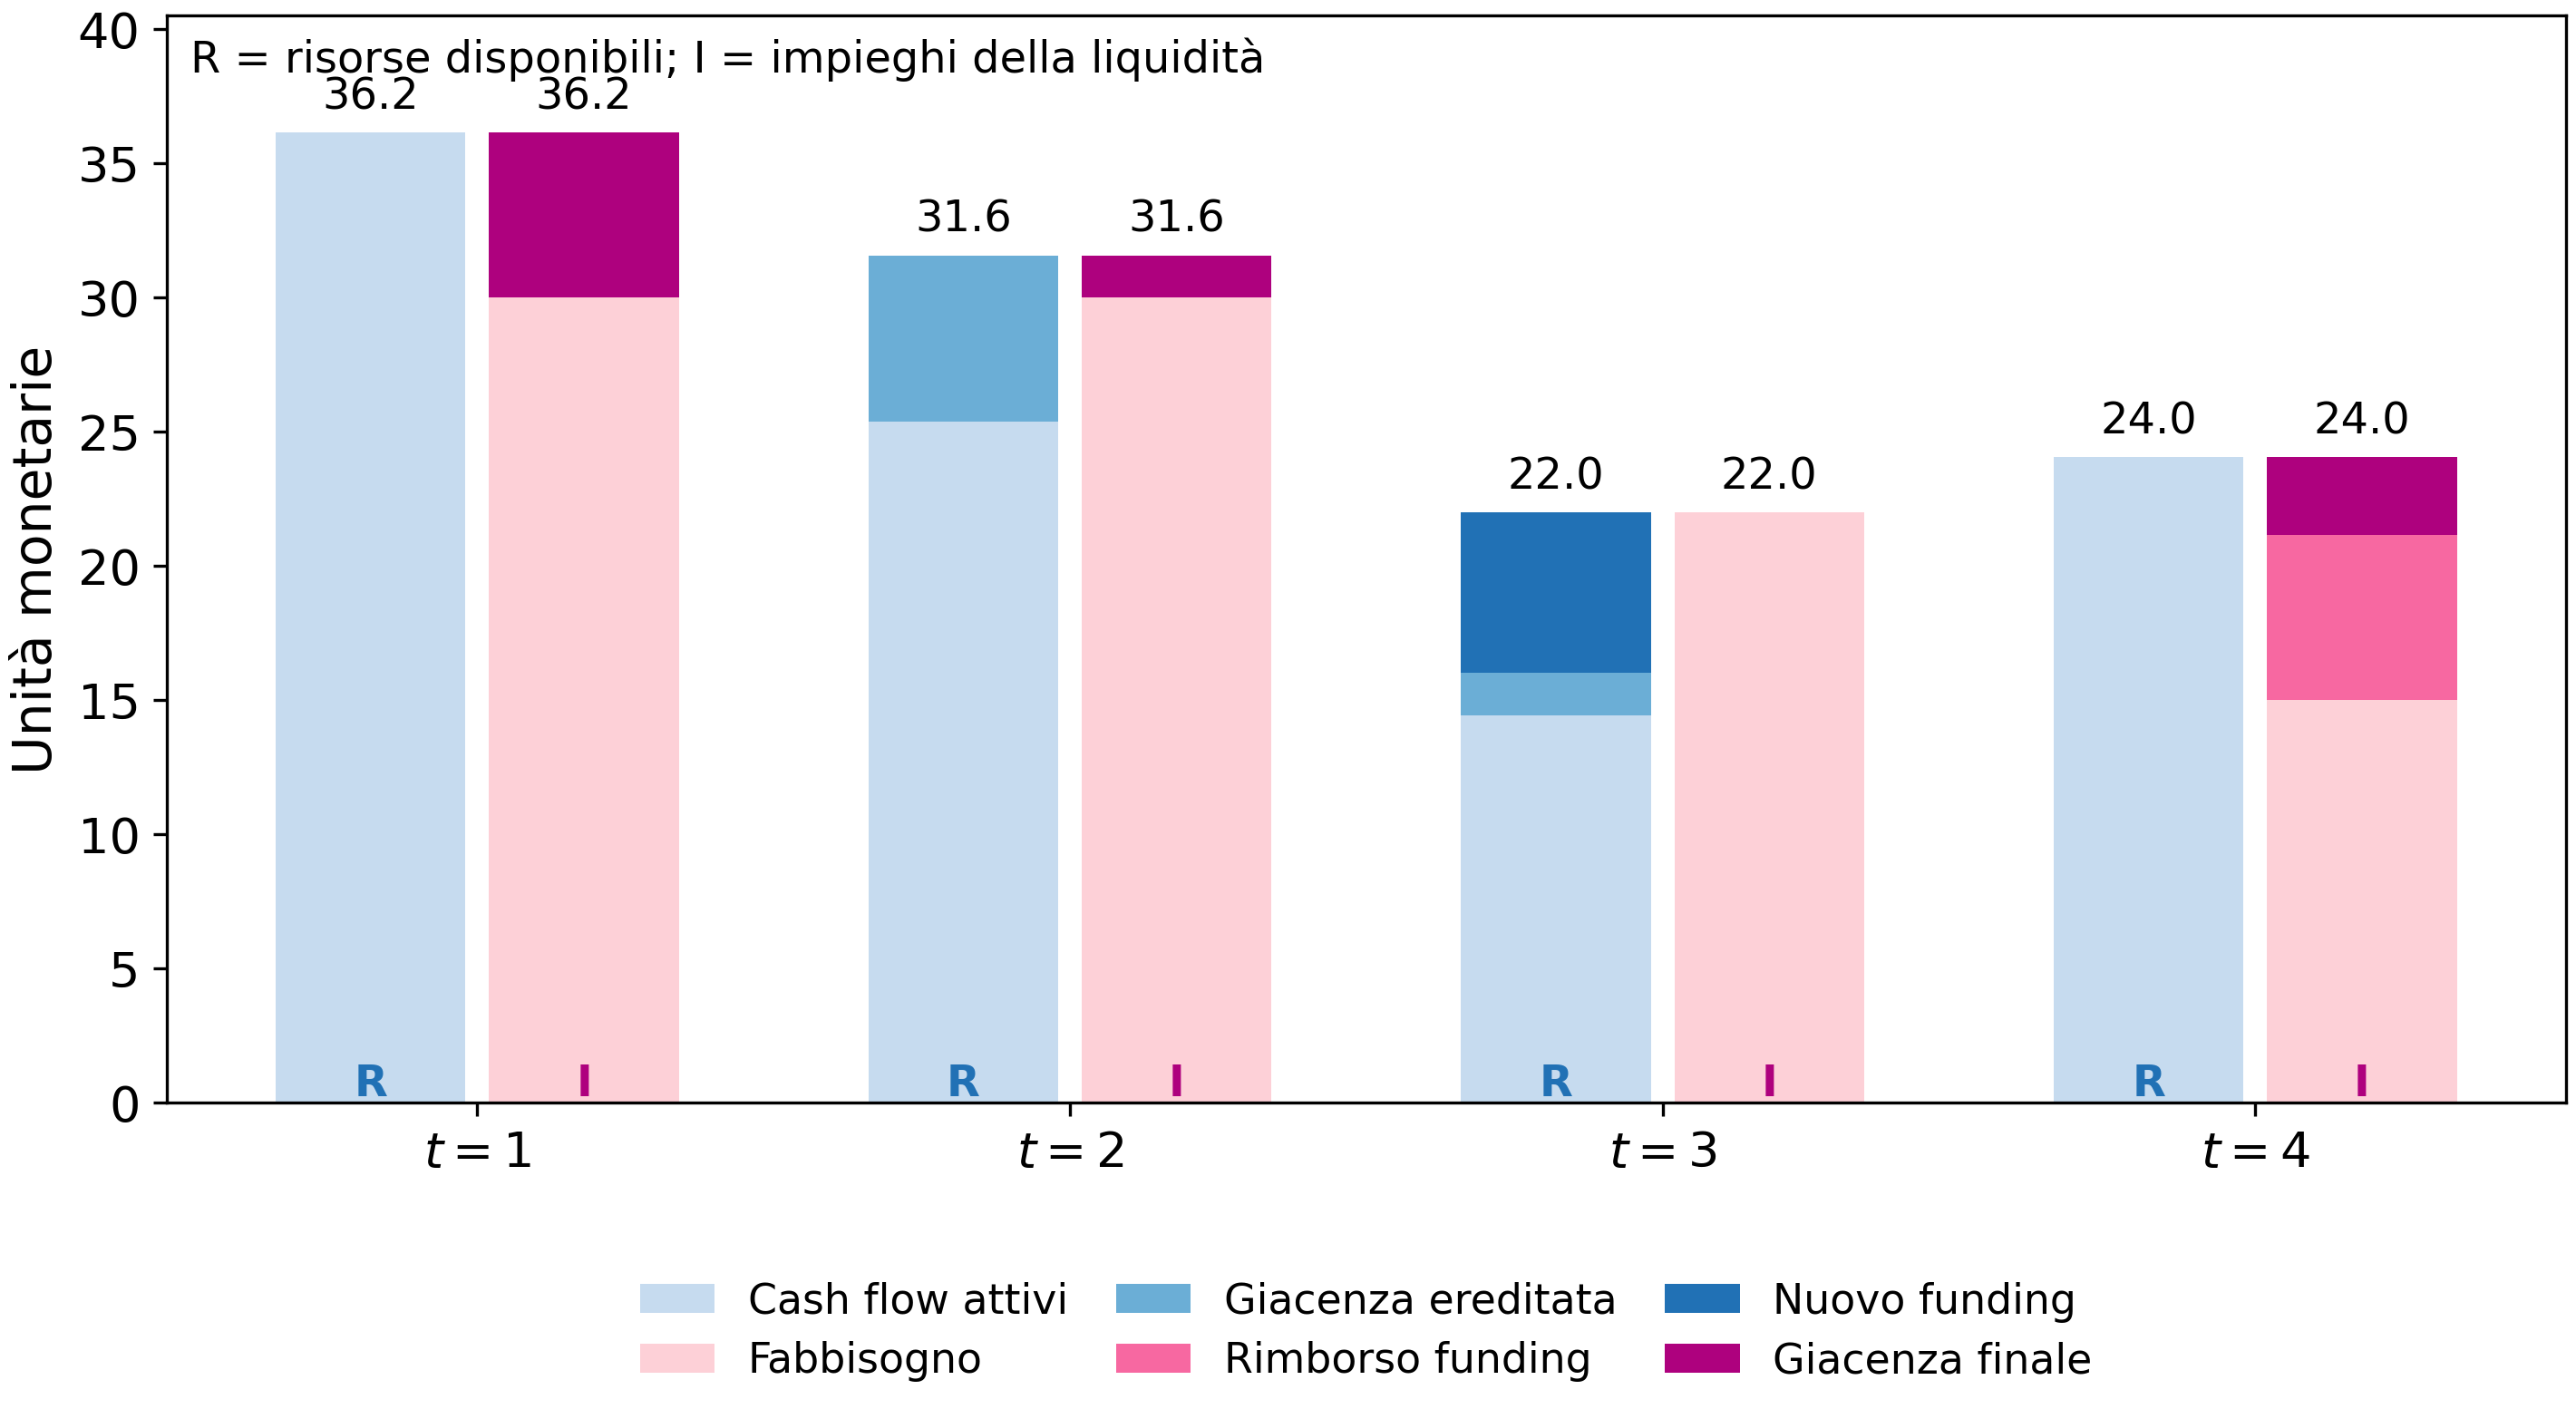
\includegraphics[width=0.78\textwidth]
{../graphics/Cap12_ALM_profili_ottimi.png}
\end{center}



%TCIMACRO{\TeXButton{Transition: Box Out}{\transboxout}}%
%BeginExpansion
\transboxout%
%EndExpansion
%TCIMACRO{\TeXButton{EndFrame}{\end{frame}}}%
%BeginExpansion
\end{frame}%
%EndExpansion

%****************************************

\subsection{Il bilancio della rinuncia}%

%TCIMACRO{\TeXButton{BeginFrame}{\begin{frame}}}%
%BeginExpansion
\begin{frame}%
%EndExpansion

\QTR{frametitle}{Quanto \`{e} costato rendere il piano finanziabile}

%TCIMACRO{\TeXButton{Transparency}{\setbeamercovered{transparent=20}}}%
%BeginExpansion
\setbeamercovered{transparent=20}%
%EndExpansion

Il risultato ottimo del modello ALM \`{e}

{\small
\[
\Pi^{*}
\approx
\underbrace{3.7020}_{c'x^{*}}
+
\underbrace{0.0402}_{\mbox{\footnotesize interessi su }g}
-
\underbrace{0.1500}_{\mbox{\footnotesize costo del funding}}
\approx
3.5922.
\]
}

\medskip

\begin{stepitemize}
\item Il confronto con $z^{*}\approx3.765$ del Capitolo~11 sarebbe per\`{o}
improprio: $\Pi$ comprende interessi (attivi e passivi) su giacenze e raccolta. Il confronto omogeneo
riguarda la sola composizione dell'attivo:

{\small
\[
c'x^{\mathrm{stat}}\approx3.765
\qquad\mbox{contro}\qquad
c'x^{*}\approx3.702.
\]
}

\item \textbf{Sei centesimi \`{e} il prezzo della finanziabilit\`{a}}: quanto
la banca rinuncia per avere un piano che sta in piedi a ogni scadenza.

\item E cambia ci\`{o} che limita la scelta. I vincoli prudenziali conservano
un margine ($\ell'x^{*}\approx4.885$ contro $7$; $x_3^{*}=0$ contro $30$),
mentre \`{e} attivo il limite alla raccolta: $u_3^{*}=\bar u_3=6$.

\item \textbf{La scarsit\`{a} si \`{e} spostata sul funding} -- ed \`{e}
l\`{i} che conviene chiedersi quanto valga una unit\`{a} in pi\`{u}.
\end{stepitemize}

%TCIMACRO{\TeXButton{Transition: Box Out}{\transboxout}}%
%BeginExpansion
\transboxout%
%EndExpansion
%TCIMACRO{\TeXButton{EndFrame}{\end{frame}}}%
%BeginExpansion
\end{frame}%
%EndExpansion

%****************************************

\section{Un prezzo per ogni scadenza}

\subsection{I valori duali dei bilanci temporali}%

%TCIMACRO{\TeXButton{BeginFrame}{\begin{frame}}}%
%BeginExpansion
\begin{frame}%
%EndExpansion

\QTR{frametitle}{Quanto vale la liquidit\`{a}, data per data}

%TCIMACRO{\TeXButton{Transparency}{\setbeamercovered{transparent=20}}}%
%BeginExpansion
\setbeamercovered{transparent=20}%
%EndExpansion


Nel Capitolo~11 un solo prezzo, $\lambda_Q^{*}$, valutava tutta la
liquidit\`{a}. Nel modello ALM ogni bilancio ha il proprio $\lambda_t^{*}$:
quanto costa alla banca un'unit\`{a} di fabbisogno in pi\`{u} a quella data.

\medskip

{\footnotesize
\[
\begin{array}{c|c|c|c|l}
\hline
t & g_t^{*} & u_t^{*} & \lambda_t^{*} & \mbox{con che cosa la banca copre }d_t\\
\hline
1 & 6.152 & 0 & 0.04524 & \mbox{solo cash flow dell'attivo; ne avanza }6.152\\
2 & 1.567 & 0 & 0.04004 & \mbox{cash flow pi\`{u} la giacenza della data }1\\
3 & 0     & 6 & 0.03383 & \mbox{esaurisce la giacenza e satura il funding}\\
4 & 2.890 & - & 0       & \mbox{copre tutto e chiude con }2.890\mbox{ di avanzo}\\
\hline
\end{array}
\]
}

\medskip

\begin{stepitemize}
\item Alle prime tre date ogni risorsa \`{e} gi\`{a} impegnata: un euro di
fabbisogno in pi\`{u} obbliga a rivedere il piano, e costa.

\item Alla data $4$ l'avanzo assorbe l'aumento senza che nulla cambi:
$\lambda_4^{*}=0$. E il fabbisogno pi\`{u} piccolo, $d_4=15$, \`{e} proprio
quello che non costa nulla.

\item \textbf{Il prezzo non misura quanto \`{e} grande il fabbisogno, ma
quanto \`{e} "stretta" la banca} nel momento in cui deve farvi fronte.
\end{stepitemize}

%TCIMACRO{\TeXButton{Transition: Box Out}{\transboxout}}%
%BeginExpansion
\transboxout%
%EndExpansion
%TCIMACRO{\TeXButton{EndFrame}{\end{frame}}}%
%BeginExpansion
\end{frame}%
%EndExpansion

%****************************************

\subsection{Come si legano i prezzi nel tempo}%

%TCIMACRO{\TeXButton{BeginFrame}{\begin{frame}}}%
%BeginExpansion
\begin{frame}%
%EndExpansion

\QTR{frametitle}{I prezzi si propagano all'indietro}

%TCIMACRO{\TeXButton{Transparency}{\setbeamercovered{transparent=20}}}%
%BeginExpansion
\setbeamercovered{transparent=20}%
%EndExpansion

\begin{center}
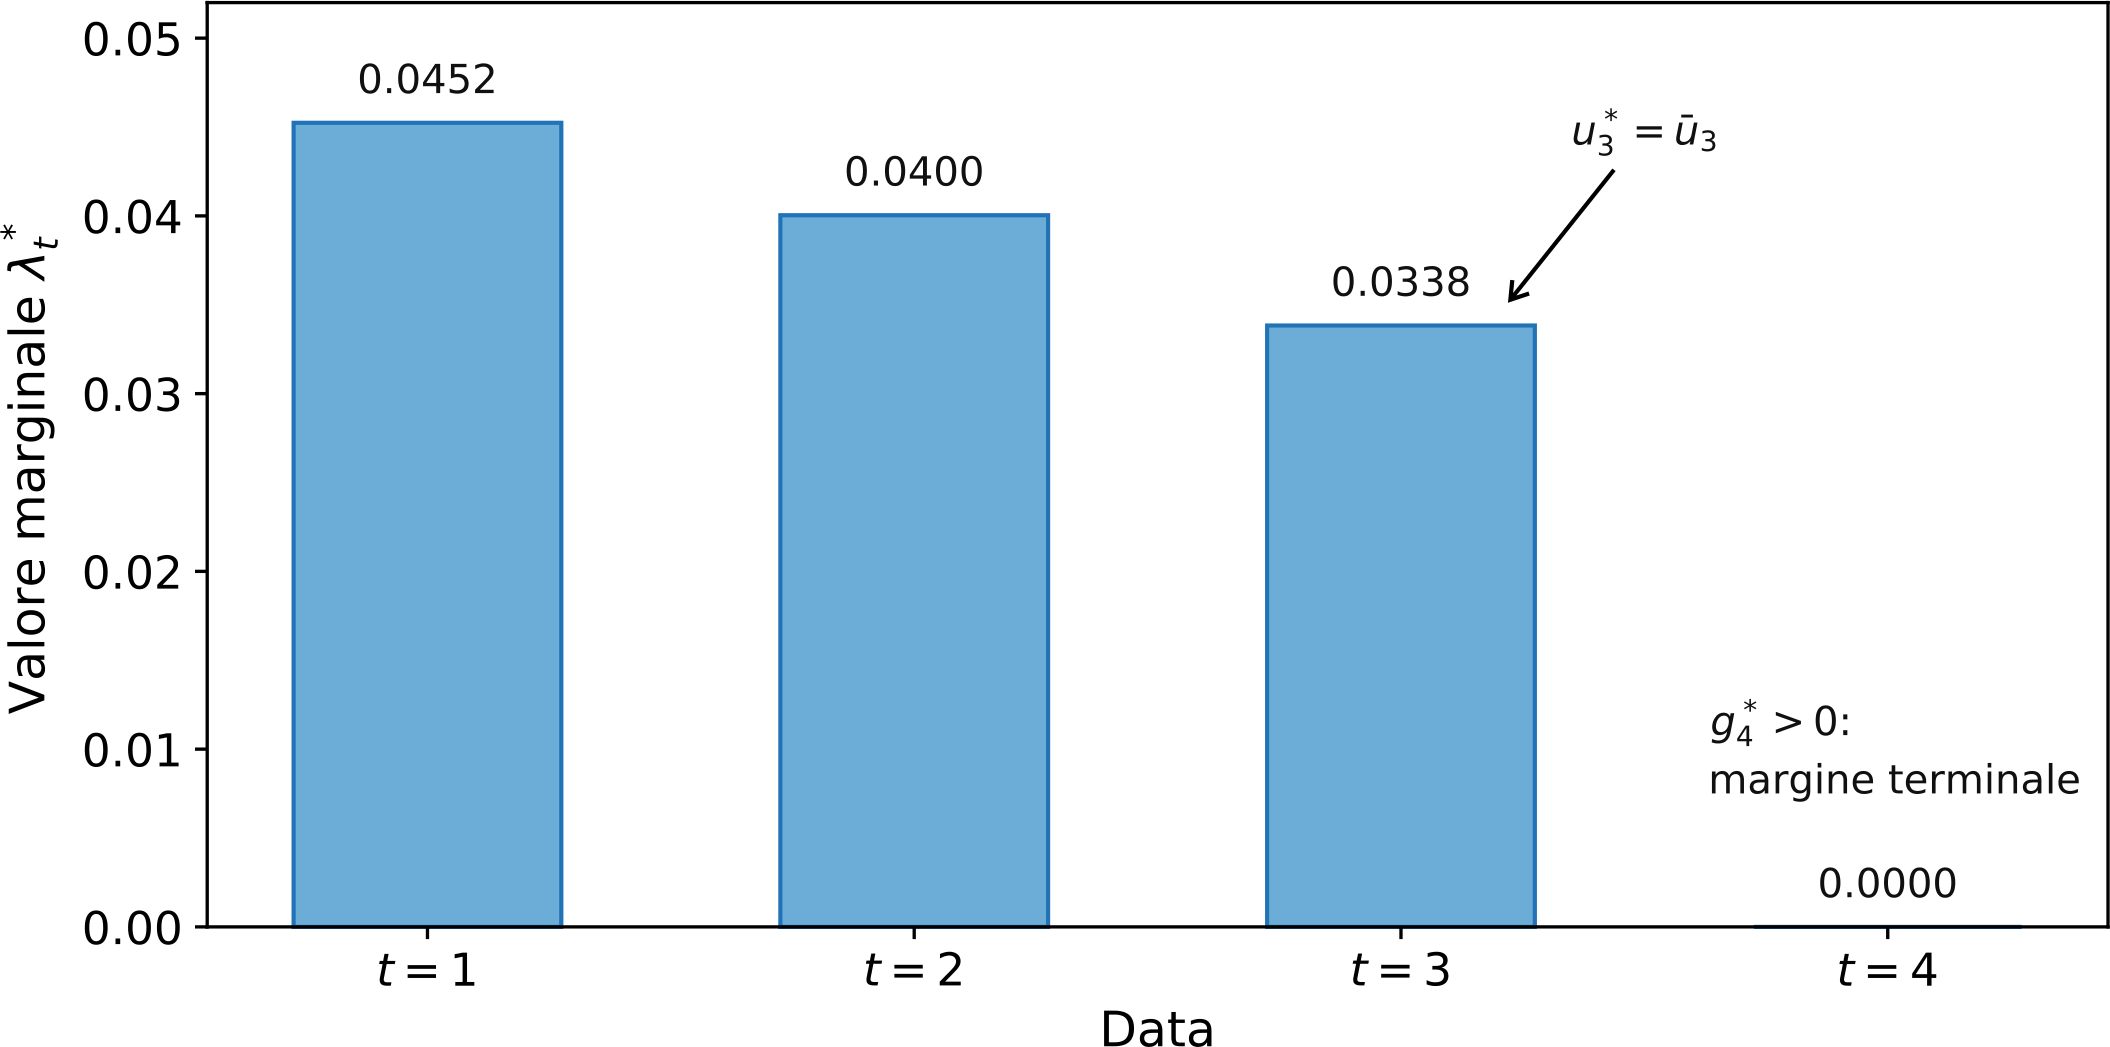
\includegraphics[width=0.62\textwidth]
{../graphics/Cap12_prezzi_ombra_scadenze.png}
\end{center}

\medskip

\begin{stepitemize}
\item Finch\'{e} la banca trasferisce liquidit\`{a} ($g_t^{*}>0$), il prezzo
di una data \`{e} quello della data successiva, capitalizzato:

{\small
\[
\lambda_t^{*}=r_t^{g}+(1+r_t^{g})\lambda_{t+1}^{*},
\qquad
0.005+1.005(0.04004)=0.04524.
\]
}

\item Il legame si spezza dove la giacenza si azzera. Alla data $3$ la banca
non pu\`{o} pi\`{u} rinviare: satura il funding, e quel limite ha a sua volta
un prezzo, $\lambda_{u,3}^{*}\approx0.00883$.
\end{stepitemize}

%TCIMACRO{\TeXButton{Transition: Box Out}{\transboxout}}%
%BeginExpansion
\transboxout%
%EndExpansion
%TCIMACRO{\TeXButton{EndFrame}{\end{frame}}}%
%BeginExpansion
\end{frame}%
%EndExpansion

\section{Esercizio in aula: interpretare i valori duali}

%****************************************

\subsection{La consegna}%

%TCIMACRO{\TeXButton{BeginFrame}{\begin{frame}}}%
%BeginExpansion
\begin{frame}%
%EndExpansion

\QTR{frametitle}{Esercizio: usare i prezzi ombra}

%TCIMACRO{\TeXButton{Transparency}{\setbeamercovered{transparent=20}}}%
%BeginExpansion
\setbeamercovered{transparent=20}%
%EndExpansion

Restiamo sul caso SVB multiperiodale, con i valori appena ottenuti:

{\small
\[
\lambda^{*}\approx(0.04524,\;0.04004,\;0.03383,\;0)',
\qquad
\lambda_{u,3}^{*}\approx0.00883,
\qquad
g_4^{*}\approx2.890.
\]
}

\medskip

\begin{stepenumerate}
\item [1.] Il fabbisogno della seconda data aumenta di $0.5$. Di quanto
peggiora il risultato?

\item [2.] La banca pu\`{o} negoziare $1$ unit\`{a} di capacit\`{a} di
funding in pi\`{u} alla terza data. Quanto vale?

\item [3.] Il fabbisogno dell'ultima data aumenta di $4$. Possiamo concludere,
da $\lambda_4^{*}=0$, che non costa nulla?
\end{stepenumerate}

\medskip

{\footnotesize Per i primi due punti si assuma che le variazioni siano
abbastanza piccole da non modificare la struttura della soluzione.}

%TCIMACRO{\TeXButton{Transition: Box Out}{\transboxout}}%
%BeginExpansion
\transboxout%
%EndExpansion
%TCIMACRO{\TeXButton{EndFrame}{\end{frame}}}%
%BeginExpansion
\end{frame}%
%EndExpansion

%****************************************

\subsection{La soluzione}%

%TCIMACRO{\TeXButton{BeginFrame}{\begin{frame}}}%
%BeginExpansion
\begin{frame}%
%EndExpansion

\QTR{frametitle}{Soluzione: i prezzi valgono solo localmente}

%TCIMACRO{\TeXButton{Transparency}{\setbeamercovered{transparent=20}}}%
%BeginExpansion
\setbeamercovered{transparent=20}%
%EndExpansion

\begin{stepitemize}
\item \textbf{Fabbisogno alla data 2.}
{\small
\[
\Delta\Pi^{*}\approx-0.04004(0.5)=-0.02002.
\]
}
Il risultato peggiora di circa due centesimi.

\item \textbf{Capacit\`{a} di funding alla data 3.}
{\small
\[
\Delta\Pi^{*}\approx0.00883(1)=0.00883.
\]
}
\`{E} il massimo che conviene pagare per quell'unit\`{a} in pi\`{u}.

\item \textbf{Fabbisogno alla data 4: no.} L'avanzo disponibile \`{e}
$2.890$, e la variazione proposta \`{e} $4$. Oltre l'avanzo il piano deve
essere rivisto, e da quel punto in poi $\lambda_4^{*}=0$ non vale pi\`{u}.
\end{stepitemize}

\medskip

{\small
\[
\boxed{
\mbox{il prezzo ombra \`{e} una pendenza locale, non un tariffario}
}
\]
}

%TCIMACRO{\TeXButton{Transition: Box Out}{\transboxout}}%
%BeginExpansion
\transboxout%
%EndExpansion
%TCIMACRO{\TeXButton{EndFrame}{\end{frame}}}%
%BeginExpansion
\end{frame}%
%EndExpansion


\section{Limiti del modello e sintesi}

%****************************************

\subsection{Che cosa significa deterministico}%

%TCIMACRO{\TeXButton{BeginFrame}{\begin{frame}}}%
%BeginExpansion
\begin{frame}%
%EndExpansion

\QTR{frametitle}{Un'ipotesi molto forte}

%TCIMACRO{\TeXButton{Transparency}{\setbeamercovered{transparent=20}}}%
%BeginExpansion
\setbeamercovered{transparent=20}%
%EndExpansion

Nel modello di oggi la banca conosce al tempo $0$ l'intera traiettoria di
$A^{\mathrm{CF}}$, $d_t$, $r_t^{g}$, $r_t^{u}$, $\bar u_t$.

\medskip

\begin{stepitemize}
\item \textbf{Deterministico non vuol dire costante}: nel caso SVB i tassi
cambiano a ogni data e la capacit\`{a} di funding si riduce, $10$, $8$, $6$.
Vuol dire che il percorso \`{e} \textbf{noto in anticipo}.

\item Per questo la banca pu\`{o} fissare gi\`{a} al tempo $0$ l'intero piano,
$u_1^{*}$ compreso -- anche se quel funding sar\`{a} raccolto fra tre
periodi.

\item Ma una banca reale decide quanto raccogliere alla data $3$
\textbf{quando arriva alla data $3$}, in base a ci\`{o} che nel frattempo ha
osservato.
\end{stepitemize}

\medskip

{\small
\[
\boxed{
\begin{array}{ccc}
u_t=\mbox{numero fissato al tempo }0
&
\longrightarrow
&
u_t=u_t(\mbox{informazione alla data }t)
\end{array}
}
\]
}

%TCIMACRO{\TeXButton{Transition: Box Out}{\transboxout}}%
%BeginExpansion
\transboxout%
%EndExpansion
%TCIMACRO{\TeXButton{EndFrame}{\end{frame}}}%
%BeginExpansion
\end{frame}%
%EndExpansion

%****************************************

\subsection{Sintesi}%

%TCIMACRO{\TeXButton{BeginFrame}{\begin{frame}}}%
%BeginExpansion
\begin{frame}%
%EndExpansion

\QTR{frametitle}{Che cosa portiamo a casa}

%TCIMACRO{\TeXButton{Transparency}{\setbeamercovered{transparent=20}}}%
%BeginExpansion
\setbeamercovered{transparent=20}%
%EndExpansion

\begin{stepitemize}
\item Il \textbf{duale} produce in una sola soluzione i prezzi impliciti di
tutti i vincoli, e la dualit\`{a} forte garantisce che valgano quanto
l'ottimo del primale.

\item La \textbf{liquidit\`{a} aggregata non basta}: la composizione ottima
del Capitolo~11 soddisfa il requisito complessivo e tuttavia non \`{e}
finanziabile alle singole scadenze.

\item \textbf{Giacenze e funding} collegano date consecutive in direzioni
opposte, e il problema resta un programma lineare.

\item Ogni scadenza ha il proprio prezzo della liquidit\`{a}, e quel prezzo
misura \textbf{quanto \`{e} stretta la banca} in quel momento.
\end{stepitemize}

\medskip

\begin{center}
{\small \emph{Chiave di lettura: la liquidit\`{a} non ha un prezzo, ne ha uno
per ogni data.}}
\smallskip

\textbf{Lezione 13}: lo stesso modello passato a un solver, in Python.

\textbf{Lezione 14}: che cosa cambia quando il futuro non \`{e} pi\`{u} noto.
\end{center}

%TCIMACRO{\TeXButton{Transition: Box Out}{\transboxout}}%
%BeginExpansion
\transboxout%
%EndExpansion
%TCIMACRO{\TeXButton{EndFrame}{\end{frame}}}%
%BeginExpansion
\end{frame}%
%EndExpansion

%****************************************
% MATERIALE DI BACK-UP
% Da inserire dopo la slide 42 e prima di \end{document}
% Le slide in appendice non entrano nella numerazione
% n\'{e} nella barra di navigazione.
%****************************************

\section{Back-up}

%TCIMACRO{\TeXButton{BeginFrame}{\begin{frame}}}%
%BeginExpansion
\begin{frame}%
%EndExpansion

\vfill
\begin{center}
{\Huge\bfseries Back-up}
\end{center}
\vfill

%TCIMACRO{\TeXButton{Transition: Box Out}{\transboxout}}%
%BeginExpansion
\transboxout%
%EndExpansion
%TCIMACRO{\TeXButton{EndFrame}{\end{frame}}}%
%BeginExpansion
\end{frame}%
%EndExpansion

%****************************************

\subsection{Dalla formulazione al solver}%

%TCIMACRO{\TeXButton{BeginFrame}{\begin{frame}}}%
%BeginExpansion
\begin{frame}%
%EndExpansion

\QTR{frametitle} {come si passa il problema a un solver}

%TCIMACRO{\TeXButton{Transparency}{\setbeamercovered{transparent=20}}}%
%BeginExpansion
\setbeamercovered{transparent=20}%
%EndExpansion

Tutte le variabili in un unico vettore, nell'ordine
$x$, poi $g$, poi $u$:

{\small
\[
v
=
\begin{pmatrix}
x_1 & \cdots & x_n &
g_1 & \cdots & g_T &
u_1 & \cdots & u_{T-1}
\end{pmatrix}',
\qquad
\max\;(c^{\mathrm{ALM}})'v,
\]
}

{\small
\[
c^{\mathrm{ALM}}
=
\begin{pmatrix}
c_1 & \cdots & c_n &
r_1^{g} & \cdots & r_{T-1}^{g} & 0 &
-r_1^{u} & \cdots & -r_{T-1}^{u}
\end{pmatrix}'.
\]
}

\medskip

\begin{stepitemize}
\item Il vincolo di bilancio iniziale e i $T$ bilanci di liquidit\`{a} sono
uguaglianze: $A_{\mathrm{eq}}v=b_{\mathrm{eq}}$.

\item I limiti prudenziali sono disuguaglianze:
$A_{\mathrm{ub}}v\leq b_{\mathrm{ub}}$.

\item I limiti sulle singole variabili completano la specificazione:
$\underline v\leq v\leq\overline v$, con $u_t\in[0,\bar u_t]$.

\item \texttt{scipy.optimize.linprog} minimizza, quindi si passa
$\widetilde c=-c^{\mathrm{ALM}}$. Metodo \texttt{highs}.
\end{stepitemize}

\medskip

{\footnotesize Il passaggio decisivo non \`{e} il solver, ma la traduzione
della descrizione finanziaria in variabili, coefficienti e vincoli.
\textbf{Lezione 13.}}

%TCIMACRO{\TeXButton{Transition: Box Out}{\transboxout}}%
%BeginExpansion
\transboxout%
%EndExpansion
%TCIMACRO{\TeXButton{EndFrame}{\end{frame}}}%
%BeginExpansion
\end{frame}%
%EndExpansion

%****************************************

\subsection{La condizione terminale}%

%TCIMACRO{\TeXButton{BeginFrame}{\begin{frame}}}%
%BeginExpansion
\begin{frame}%
%EndExpansion

\QTR{frametitle}{che cosa fare della liquidit\`{a} finale}

%TCIMACRO{\TeXButton{Transparency}{\setbeamercovered{transparent=20}}}%
%BeginExpansion
\setbeamercovered{transparent=20}%
%EndExpansion

La variabile $g_T$ non \`{e} un residuo tecnico: dichiara che cosa il modello
considera economicamente rilevante alla fine dell'orizzonte.

\medskip

{\footnotesize
\[
\begin{array}{l|l|l}
\hline
\mbox{scelta} & \mbox{significato} & \mbox{effetto su }\lambda_T^{*}\\
\hline
g_T=0
& \mbox{nulla deve avanzare}
& \mbox{in generale }\lambda_T^{*}\neq0\\
g_T\geq0\mbox{, non valorizzata}
& \mbox{l'avanzo \`{e} ammesso ma non premiato}
& \lambda_T^{*}=0\mbox{ se }g_T^{*}>0\\
g_T\mbox{ nell'obiettivo}
& \mbox{l'avanzo ha valore oltre l'orizzonte}
& \mbox{riflette quel valore}\\
\hline
\end{array}
\]
}

\medskip

\begin{stepitemize}
\item Nel caso SVB abbiamo adottato la seconda: $g_4^{*}\approx2.890$
\`{e} ammesso e non premiato, e infatti $\lambda_4^{*}=0$.

\item \textbf{Il prezzo nullo dell'ultima data non \`{e} una propriet\`{a}
dell'ALM}: dipende da questa scelta. Con $g_T=0$ imposto, l'ultima data
avrebbe un prezzo come le altre.

\item Se la banca prosegue l'attivit\`{a} oltre $T$, forzare $g_T=0$ \`{e}
economicamente improprio: l'orizzonte del modello non \`{e} la fine della
banca.
\end{stepitemize}

%TCIMACRO{\TeXButton{Transition: Box Out}{\transboxout}}%
%BeginExpansion
\transboxout%
%EndExpansion
%TCIMACRO{\TeXButton{EndFrame}{\end{frame}}}%
%BeginExpansion
\end{frame}%
%EndExpansion

%****************************************

\subsection{Dualita debole}%

%TCIMACRO{\TeXButton{BeginFrame}{\begin{frame}}}%
%BeginExpansion
\begin{frame}%
%EndExpansion

\QTR{frametitle}{perch\'{e} il duale sta sempre sopra}

%TCIMACRO{\TeXButton{Transparency}{\setbeamercovered{transparent=20}}}%
%BeginExpansion
\setbeamercovered{transparent=20}%
%EndExpansion

Siano $x$ ammissibile per il primale ($Ax\leq b$, $x\geq0$) e $\lambda$
ammissibile per il duale ($A'\lambda\geq c$, $\lambda\geq0$).

\medskip

{\small
\[
c'x
\;\underbrace{\leq}_{A'\lambda\geq c,\ x\geq0}\;
(A'\lambda)'x
=
\lambda'Ax
\;\underbrace{\leq}_{Ax\leq b,\ \lambda\geq0}\;
\lambda'b
=
b'\lambda.
\]
}

\medskip

\begin{stepitemize}
\item Due sole disuguaglianze, ciascuna ottenuta moltiplicando un vincolo per
un vettore non negativo. Nessun'altra ipotesi.

\item Conseguenza: \textbf{ogni} soluzione duale ammissibile fornisce un
limite superiore al primale, e viceversa.

\item Se per una coppia ammissibile risulta $c'x=b'\lambda$, allora
\textbf{entrambe sono ottime}: non serve risolvere per saperlo.

\item La dualit\`{a} \emph{forte} aggiunge che quella coincidenza si verifica
sempre, quando l'ottimo esiste finito.
\end{stepitemize}

%TCIMACRO{\TeXButton{Transition: Box Out}{\transboxout}}%
%BeginExpansion
\transboxout%
%EndExpansion
%TCIMACRO{\TeXButton{EndFrame}{\end{frame}}}%
%BeginExpansion
\end{frame}%
%EndExpansion

%****************************************

\subsection{Ambiente esterno e stato interno}%

%TCIMACRO{\TeXButton{BeginFrame}{\begin{frame}}}%
%BeginExpansion
\begin{frame}%
%EndExpansion

\QTR{frametitle}{l'ambiente economico-finanziario}

%TCIMACRO{\TeXButton{Transparency}{\setbeamercovered{transparent=20}}}%
%BeginExpansion
\setbeamercovered{transparent=20}%
%EndExpansion

Le tre componenti di $\bar Z_t=(\bar Z_t^{R},\bar Z_t^{C},\bar Z_t^{F})$
hanno funzioni economiche distinte:

\medskip

{\small
\[
\begin{array}{l|l|l}
\hline
\bar Z_t^{R} & \mbox{livello dei tassi privi di rischio} & \mbox{prezzo del tempo}\\
\bar Z_t^{C} & \mbox{spread di credito di mercato} & \mbox{prezzo del rischio di credito}\\
\bar Z_t^{F} & \mbox{tensione sul funding della banca} & \mbox{prezzo della scarsit\`{a} di funding}\\
\hline
\end{array}
\]
}

\medskip

\begin{stepitemize}
\item Da qui i coefficienti: $r_t^{g}=r^{g}(\bar Z_t^{R})$,
$r_t^{u}=\bar Z_t^{R}+\bar Z_t^{F}$, $\bar u_t=\bar u(\bar Z_t^{F})$. Se
$\bar Z_t^{F}>0$, allora $r_t^{u}>r_t^{g}$.

\item $\bar Z_t^{C}$ entra nei cash flow \textbf{solo se} i flussi
dipendono dalla qualit\`{a} creditizia: perdite attese, valori di realizzo,
haircut. Non per il solo fatto che il modello contiene un fattore di credito.

\item Le decisioni retroagiscono sullo stato:
$X_{t+1}=G(X_t,u_t,\bar Z_t,d_t)$. Il funding di oggi peggiora la posizione
di domani; la giacenza la migliora.

\item \textbf{Deterministico} significa che l'intera traiettoria
$\bar Z_0,\ldots,\bar Z_T$ \`{e} nota al tempo $0$ -- non che sia costante.
\end{stepitemize}

%TCIMACRO{\TeXButton{Transition: Box Out}{\transboxout}}%
%BeginExpansion
\transboxout%
%EndExpansion
%TCIMACRO{\TeXButton{EndFrame}{\end{frame}}}%
%BeginExpansion
\end{frame}%
%EndExpansion





%****************************************
\end{document}